\chapter{Старинные источники}

Попробуем копнуть прошлое земель от Воскресенки до Троещины подробнее, по доступным документам. Долгое время, около столетия, редким печатным источником таковых была статья, на деле доклад члена киевского церковно-археологи\-ческого общества Виктора Гошкевича «Замок князя Симеона Олельковича и летописный Городок под Киевом», читанный в заседании общества 18 сентября 1889 года и опубликованный в «Трудах Киевской духовной академии» во втором выпуске за год 1890-й.

Когда Екатерина II отбирала у церкви земли в казну, давние жалованные грамоты и универсалы с указаниями границ и урочищ попали из киевских монастырей в Казенную палату. Десятилетия спустя, митрополит Евгений Болховитинов нашел там эти документы и, как сообщает Гошкевич, «передал на хранение в библиотеку Киевской Духовной Академии».

С документами много поработал профессор Николай Петров, крестный отец Михаила Булгакова. Частью они были опубликованы Императорской Археографической Комиссией, рассеявшись по многочисленным томам «актов», относящихся к истории Западной и Юго-западной Руси, да подобным сборникам. Но большинство осталась молчаливо лежать в закромах. 

«Благодаря любезности проф. Петрова, я имел возможность заняться разработкой этого архивного матерьяла», – загадочно пишет Гошкевич, подразумевая то ли заслуги Петрова по упорядочению архива, то ли просто допуск к документам.

Гошкевич посулил общественности большую краеведческую работу на основе этих бумаг, однако по незавершенности ея решил сначала поделиться более коротким исследованием, посвященным городищу двора Олельковича и связанным с ним источникам. Первое своё обещание он так и не выполнил, в том же году или вскоре переехав в Херсон, где закрутилась новая жизнь – издание газеты «Юг» и устроение местного музея, ныне Херсонского областного краеведческого музея.

\begin{center}
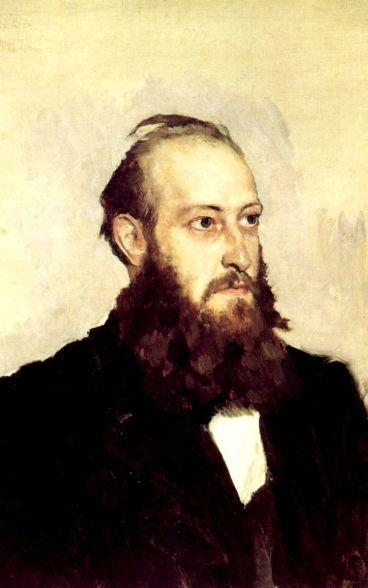
\includegraphics[width=0.55\linewidth]{chast-gorodki/star-ist/goshkevich01.jpg}

\textit{Виктор Гошкевич. Портрет работы Виктора Васнецова.}
\end{center}

В Киевской Духовной Академии было два брата Гошкевича – старший Осип (Иосиф) Антонович, да отец Виктора, протоиерей Иоанн Антонович, преподаватель логики, психологии и латинского языка, догматического и нравственного богословия, настоятель Царе-Константин\-овской церкви. Он умер в 1871 году, когда Виктору исполнилось 11 лет.

Закончив Духовную семинарию, Виктор в 1881 году поступил в Киевский университет, на  математический и историко-филологический факультеты. Там же участвовал в кружке Владимира Бонифатьевича Антоновича.

Историю искусств преподавал профессор А. В. Прахов, заведовавший росписью Владимирского собора. Через Прахова с Гошкевичем познакомился Виктор Васнецов и списал с него этюд, использовав оный для воплощения фигуры Моисея в росписи алтарной части храма. Напомню, что голова художника Светославского послужила моделью васнецовского Моисея на фронтоне, на фреске Преображения Господнего.

Вместе с Петровым Гошкевич устроил в Лавре Музей Цер\-ковно-археологического общества. В Херсон же перебрался следом за братом своим Михаилом, на должность секретаря губернского статистического комитета. Уже в 1902 году вышла книга Виктора Ивановича «Клады и древности Херсонской губернии».

При советской власти он продолжил свою археологическую и краеведческую деятельность с уклоном в юг Украины, а умер в 1928 году, лишь на семь лет пережив Петрова. Похоронили Гошкевича в Херсоне на городском кладбище, позже могилу перенесли в усадьбу Краеведческого музея.

А прах Петрова был предан земле Флоровского кладбища, на Замковой горе. Осквернен и сгинул! Какие толковые люди собрались в конце 19-го, начале 20 веков в Киевской Духовной академии, и как стёрся след их с лица земли. Завитневич, Петров, Лебединцев\footnote{Петр Гаврилович Лебединцев (1819-1896). Брат его, историк Феофан Гаврилович (1828-1888), был первым редактором «Киевской старины». Оба похоронены на застроенном ныне Щекавицком кладбище (не-старообрядческом).}.

Пара-другая документов про окрестности Выгуровщины и Троещины была опубликована в разрозненных книжках и статьях, а в 2011 году в Киеве тиражом 200 экземпляров вышел сборник «Документальное наследие Свято-Михайловского Златоверхого монастыря в Киеве»\cite{mihdocs}.

Различные земельные грамоты, протоколы комиссий размежевания, купчие. Обсудим и попробуем соотнести с современным рельефом.

В первую очередь важны описания границ, а границы состоят из промежутков между точками. Точками служат урочища – поименованные части местности.

При таком способе ограничивания (а он применяется поныне\footnote{Например, в описании границ охранной, заповедной археологической зоны, хотя думаю точнее было бы отметить границу на плане местности и утвердить такую графическую границу, а не словесную.}, но существуют карты), о сохранении точности границ на протяжении веков не может быть и речи, ведь водоемы переменяют русла, исчезают, деревья вырубаются, и так далее. Наконец, сами названия прыгают с места на место. 

Недавний пример – переход названия Юрковицы с отрога Щекавицы на соседнюю Лысую гору. Немудрено, что возникали земельные споры, и при каждом вызывали в свидетели старожилов, у коих выясняли, где находятся упомянутые в документах урочища. От показаний старожилов и зависел исход спора.

Перед разбором давних документов напомню о взаимном расположении сел Выгуровщины и Троещины прежде 1877 года, когда последнюю перенесли восточнее от берега русла, что ныне зовется Десенкой и Черторыей. «Старой» Троещине на 2017 год соответствуют залив Доманя\footnote{50°31'42"N 30°34'10"E} и пространство от него на восток к строящемуся коттеджному городку.

Впрочем неясно, первое ли это перемещение села Троещины, однако поскольку мне неизвестны другие перемещения, буду предполагать, что в разбираемых далее документах Троещина занимает то же место, какое занимала до 1877 года.

\begin{center}
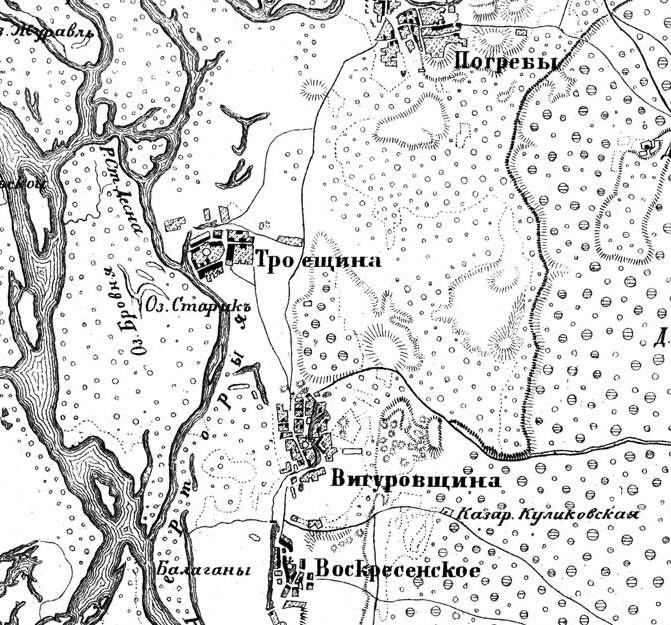
\includegraphics[width=\linewidth]{chast-gorodki/star-ist/1850.jpg}

\textit{Кусочек карты 1850 года.}
\end{center}

При киевском воеводе Андрее Якубовиче Немеровиче, состоящего на этой должности в 1511-1523 годах\footnote{В том же 1523 году Немерович получил от короля Жикгимонта I Старого привелей на предоставление прав игумену Макарию на восстановление Михайловского Златоверхого монастыря, пребывавшего тогда в запустении. Привелей указывал на передачу игумену зданий монастыря, чтобы тот отстроил их и возродил монашескую общину. Возобновлялись права на землевладения вокруг монастыря – по Пробитый вал и под Ляшские ворота, по Евсейкову долину, по старую дорогу, по Михайловский узвоз.}, в ходе разбора земельного спора между Троицким монастырем и жителями Милославщины, что принадлежала киевскому замку, четко положили границы некоему землевладению. У Гошкевича неясно\footnote{Следует помнить, что «Труды Киевской Духовной академии» издание всё-таки церковное. Доклад Гошкевича затрагивал спорные вопросы между вполне современными ему монастырями, поэтому, думаю, не случайны некоторые недомолвки в изложении и сокращения в выдержках из документов.}, чьим оно было – Троицкого или Михайловского монастыря, хотя в статье запев такой: «в документах Троицкого монастыря есть прямое указание, что местность нынешней Троещины уже принадлежала этому монастырю в первой четверти XVI века», однако первые же строки описания границы противоречат сказанному, ибо документ гласит: «почавши нижей \textbf{села их} Милославского», а Милославское было замковым, потом Викгуры, потом Михайловского монастыря!

Для удобства, здесь и далее описания границ разбиваю на пункты:

\begin{quotation}
1. Почавши нижей села их Милославского з Днепра через речку Радунку,

2. а оттою долиною ку кладовищу,

3. а от кладовища подле борку, к городищу прежднему где бил двор князя Семена Олелковича\footnote{После смерти его прошло тогда около 40 лет. Правил же Киевом Олелкович в 1455-1470 годах.}, 

4. а от того городища там же подле борку в прудец,

5. а от прудца долиною живцом около стойла на конец кривой нивы, аж у речку Угнор,

6. и тим Угнором к полю,

7. а от поля ку красному\footnote{Красивому.} дубу тим же Гнором,

8. а от красного дуба живцом у залозное озеро,

9. а от того озера у Десну ку Бокланскому острову и к верхнему концу

10. а оттоль наниз Десною округ Калинова рогу также до Днепра до того ж местца.
\end{quotation}

Это определение будет дополняться и меняться в последующие столетия. Пока же, отринув другие источники, истолкуем этот.

1. Граница проходила ниже (на юг от) села Милославского, от Днепра через речку Радунку. Из этого не следует, что Радунка вытекает из Днепра, просто граница длится от Днепра, а затем по некой местности доходит до Радунки и далее следует «через» нее.

Но при чем тут Днепр? Сейчас, ближайшее к Выгуровщине на запад речное русло принадлежит Черторые, на берегу которой стояла до 1877 года и Троещина, однако на время рассматриваемого документа села Троещины не существовало. Что же думать, исходя из грамоты?

Что где-то южнее Милославского села (позже там возникло село Выгуровщина) была речка Радунка, перейдя которую, долиной можно было добраться до кладбища «подле борку».

А что до русла, занятого ныне Черторыей... Черторыя не упомянута. Поскольку следующим после Днепра водоемом на восток названа Радунка, можно предположить, что на описываемой широте Радункой называлось русло, ныне именуемое Десенкой и Черторыей, либо же какой-то другое русло.

Полагаю, в какое-то время, быть может и в 16 веке, руслом Радунки были, кроме прочего, нынешние русла Гнилуши и озера Радунки. А начиналась речка Радунка около Погребов, на северо-восток от современного истока Черторыи (что близ устья Десны).

2. От Радунки – долиной ко кладбищу. Долиной речки ли Радунки?

3, 4 – «а от кладовища подле борку, к городищу прежднему где бил двор князя Семена Олелковича, а от того городища там же подле борку в прудец».  

Четыре смежных урочища – кладбище, борок, городище двора Олельковича, прудец. 

Уже на начало 16 века княжеского никакого двора не существовало, были какие-то остатки, «городище», слывшее тем, что осталось от двора. 

Ученые связывают место «городища», помимо замка Олельковича, с летописным Городком. Я пока намеренно не касаюсь этих вопросов, мы еще недостаточно хорошо изучили местность и истории находок на ней.

Прудец – будущий «Прудок», здесь это, кажется, обычный пруд, откуда «живец» – ручей соединял Прудец и Угнор. Мне удобно считать, что Прудец или Прудок – запруженная и потому расширенная часть речки Угнор.

Раньше я предполагал, что Прудок или Прудец для земельных грамот название странное, ведь на «роськой мове» Княжества Литовского пруд обозначался словом «став», «ставок». Однако в одном документе 18 века я встретил выражение «поуз тот Юрков прудок дорога спорчена», и это поколебало следующие мои домыслы, а именно – названия писали на бумагу со слуха. «Б» звучит как «п», может было «бруд» (грязь), «брудок». Если русло было в торфяной почве или текло с болото, конечно вода была грязной, брудной.

Другой вариант – «пруд», «прудок» – прежнее «брод», «бродок». 

А может, «прудок» это искаженное «порудок», «по руде» – в отдельной главе я поведаю о залежах болотной руде возле Выгуровщины.

Слово же «Угнор» или «Гнор» я вообще нигде более не встречал и не понимаю его значения.

Забегая вперед рассматриваемого документа, расскажу следующее.

В работе Ивана Парникозы «Киевские острова и прибрежные урочища на Днепре – взгляд сквозь века» был приведен кусками план владений Пустынно-Никольско\-го монастыря за 1719 год, там все окрестности Выгуровщины подписаны, да прочесть удается лишь некоторые.

Между Выгуровщиной и Воскресенкой показано прямое, как вытянутый питон, «верховье речки Пруда». Эдак с юго-востока в него впадает, с виду равнинная река, подписанная как «болото Убедь». Село Выгуровщина нарисовано на северном берегу Прудка, и по тому же берегу, восточнее, лежит «урочище Глинище» (верно ли прочтение?).

Русло Черторыи (на куске карты видно, что оно исходит из Днепра, ближе к нынешнему устью Десны, но Десна и устье ее лежат вне фрагмента карты) обозначено как «река Черторой», чуть севернее Выгуровщины туда впадает короткая «речка», чье название явно начинается с «р», а далее не разобрать, может таки «радунка». Речка Пруд, южнее Выгуровщины, разделяется надвое. Один рукав впадает в Черторыю, другой же следует на юг даже мимо Воскресенки, вероятно по руслам Гнилуши и озера Радунки, а подписан этот рукав «речка Ми...». 

Я списался с Парникозой и он любезно прислал мне сканы в лучшем качестве, однако и там ничего я разобрать не смог.

Вот название рукава:

\begin{center}
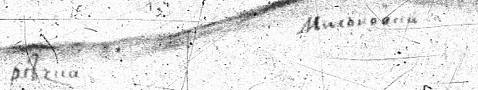
\includegraphics[width=\linewidth]{chast-gorodki/star-ist/1719-01.jpg}
\end{center}

А вот название острова или озера между ним и руслом, подписанным на карте как Черторыя:

\begin{center}
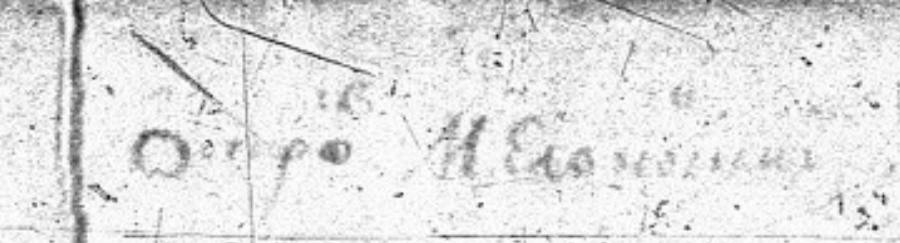
\includegraphics[width=\linewidth]{chast-gorodki/star-ist/1719-02.jpg}
\end{center}

Обе надписи кажутся мне похожими. Зная, что в тех краях была речка Меленовка и остров Меленовский, можно сопоставить речку «на букву М» с Меленовкой, и тогда Меленовкой названо русло, занимаемое ныне Гнилушей и продолжавшееся вдоль Воскресенки как озера Радунка и Меленовка (оба, вероятно, рукава одной речки). Другой вариант – М как-то связана с Михайловским озером, островом и местностью Михайловщиной, владениями Михайловского Златоверхого монастыря. Вариант третий – надпись на второй картинке означает «М.» (малый, малая) «Е.....».

%План, казалось бы, опровергает мои рассуждения о том, что Десенка это сместившаяся речка Радунка, поскольку Радунка тут оказывается вообще крошечной речкой севернее Выгуровщины, а русло того, что я полагаю Радункой, занимает речка на букву «М».

Не будем забывать, что между планом и разбираемым документом с описанием границ лежат почти две сотни лет, за которые названия водоемов (как и сами водоемы) могли измениться. Хотя на плане 1719 года Радунка показана огрызком севернее села Троещины (до 1877 года, как вы помните, оно было на берегу Черторыи), нельзя закрыть глаза на то, что озеро Радунка всё же называется именно так, а не иначе, и что Черторыи в документе нет, и что в «почавши нижей села их Милославского з Днепра через речку Радунку» слово «нижей» означает «южнее», стало быть во время составления документа речка Радунка протекала кроме прочего и южнее Выгуровщины, а значит и Троещины.

Что до Угнора, то М. Рыбаков в статье 1990 года «Вигурівщина-Троєщина – околиця Києва» приводит выдержку из документа 1780 года о происхождении села Выгуровщины, что прежде это было

\begin{quotation}
вольное местечко или городок под названием Милославск, в котором жительствовали сотни Киевской казаки и мещане, а по завладению оною мещане еще задержано, короны польской земянином Яном Вигурою переименовано в Вигуровщину. Но в каком где году так как иногда оное и кем первоначально осажено за держание, знать не можно […] Замок в окружности 221 три аршинных сажени, село простирается по обеим сторонам речки Угнор окружностью 1600 саженей таких же […] на левой стороне реки Днепра против самого города Киево-Подола.
\end{quotation} 

Поскольку, по источникам, Выгуровщина лежала по обеим сторонам водоема Прудка, что соединялся ручьем с Угнором, следует – Прудок это часть Угнора и есть.
 
Но вернемся к ограничению земель начала 16 века.

С «борком» (пункт 3) я носился года полтора, полагая, что в документе слово значит не уменьшительное от «бор», то бишь не соснячок, а в смысле, записанном даже в словаре Даля: «гробовище, могилки, земля родительская или священная, кладбище, погост, жальник».

Но потом я стал встречать в земельных документах многочисленные «борки» и понял, что ошибался.

% Хотя чертовски жаль отказывается от первого толкования, ведь находка Завитневича, полукруглый погребальный вал – отнюдь не следы имения князя Олельковича или же Городка – удачно вписывались в такую трактовку.

%Но моя ошибка не снимает вопрос. Известное археологам «городище», а на деле погребальный комплекс, на восточном берегу Гнилуши – это не городище Олельковича. Значит, последнее просто было рядом, либо вал ошибочно считали неким городищем двора Олельковича.

Пятый пункт, вернемся к нему – от Прудца «долиною живцом около стойла на конец кривой нивы, аж у речку Угнор». Стойло, оно же Стуйло – как увидим далее, название урочища, как и кривая нива. Про Стуйло известно еще, что оно было «над» болотом Корчевней, значит северней его. Корчовня или Корчевня находилась между улицей Кибальчича и проспектом генерала Ватутина.

Пункты шестой и седьмой я пропускаю, ибо уже не сыщешь того поля, к коему граница шла Угнором, а красный дуб давно исчез. В восьмом пункте упомянут живец (ручей) в «залозное озеро». Залозное – за лозами или железное?

Из девятого пункта очевидно, что озеро было уже близко к Десне и «Бокланскому острову» на ней.

Пункт десятый: «а оттоль наниз Десною округ Калинова рогу также до Днепра до того ж местца» – Калинов рог сохранился на карте лоций 1914 года как урочище Калиновка на северо-восточном углу острова Муромец. Сейчас Калиновку омывает с севера – Десна, с востока – Черторыя.

Продолжим рассматривать документы.

Жалованная грамота Киевского воеводы, князя Константина Константиновича Острожского Михайловскому Златоверхому монастырю на владения, от генваря 12, года 1560:

\begin{quotation}
Я Костентин Костентинович Острозский, воевода Киевский, маршалок Волынское земли, староста Володимирский. 

Били нам челом богомолцы господарские, игумен монястыря светого Михайла Золотоверхого, отец Семен, и вси чернцы того манастыря, абыхмо им дали островок Обрубный за рекою за Днепром, на верхнем концы Черторыи, зо всим и на все, яко ся тот островок з давных часов у себе мает, з озером Петриковом и Плоским, и Жерело Тысяцкое, и с сеножатми, поченши речкою Радункою от верхнего конца, аж до нижнего речки Радунки у Чорторыю, а другим краем к Днепру, который они от часов немалых за предков наших спокойне держали.
\end{quotation}

Верх и низ в грамотах означают север и юг. Про Радунку тут сказано, что ее южный конец смежен с Черторыей. При этом островок Обрубный – в «северном конце» Черторыи. Значит он где-то на стыке Радунки и Черторыи.

Островок Обрубный описан как «за рекою за Днепром, на верхнем концы Черторыи». Значит, на время составления документа, в северной точке Черторыи, стало быть в ее истоке, был островок Обрубный.

Еще выше, по документу, лежит речка Радунка. Она впадала в водоем, именовавшийся тогда Черторыей. Такое возможно лишь в случае, если Черторыя в то время начиналась как рукав Днепра, пробившийся к Радунке.

Озеро Плоское – возможно то же, что «болото Плосское» на лоциях 1914-го, изображенное напротив северной части озера Радунки, между нею и Неводным. Юго-восточнее Неводного на той же карте – урочище Михайловский луг, а ведь в грамоте говорится именно о владениях Михайловского монастыря.

Из «Подтвердительной грамоты короля Сигизмунда Августа, признающей право владения Киевскому Михайловскому Золотоверхому монастырю на разныя земли и угодия приобретенные им», 1570, июня 4:

\begin{quotation}
затон Пустый, который на верх Немкоцы с сеножатью по жерело Тысяцкое, и по Городовое озеро, и по речку Радунку и по Чорторыю; а от Жерела Тисяцкого на левую сторону ку Днепру
\end{quotation}

Городовое озеро мне сложно с чем-либо сопоставить, как и Тысяцкое жерело.

% По совокупности данных, руководствуясь краеведческим чутьем, я догадываюсь, что еще в 16 веке Черторыей слыл рукав Днепра, который начинался около урочища Черторыя, примерно в месте, где теперь соединяются острова Труханов и Муромец – примерно около Петровского железнодорожного моста, несколько выше.

%А южнее, в протяженности нынешних Русановских садов, в этот рукав Днепра впадала Радунка. Каким из русел – тем восточным, от коего остались озера Гнилуша и Радунка, или западным, чьи остатки – озера Неводное и Русановское, я не знаю.

Смежные с Обрубным островом урочища всплывают из пучин истории в документе, без даты напечатанном в прибавлениях к Киевским епархиальным ведомостям\cite{kieparhprib01} – сказано лишь, что границы местности Михайловщины (судя по названию, те же владения Михайловского монастыря) описаны так (разбиваю на пункты):

\begin{quotation}
1. от поля федоровского, названаго монастырского, над речкою Радункою\footnote{На электронной карте Визикома за 2006 год, где иногда всплывают редкие названия урочищ, отмечено «урочище Федоркивщина» на западной стороне улицы Пуховской – поле сразу на север от монетного двора. Координаты: 50°30'53"N 30°38'20"E. Это возле Алмазного озера, однако далековато до Черторыи и Радунки (в ее предполагаемом мною положении). Оттуда до озера Гнилуши – около 4,5 километра, то есть нельзя сказать, чтобы поле было над Радункой, если Гнилуша это часть русла Радунки.},

2. Чорториею мимо желтые воды, на острове ж Михайловском стоячие. 

3. Черториею идучи в низ мимо остров Кодак до Водохового перевалу; 

4. от Водохового перевалу повернувши в лево в речку Гнилушу до озера Неводному, належачого до того ж острова Михайловского, 

5. подле того ж озера Гнилушою идучи в гору в лево Михайловский остров, а в право остров Городовый Богарский.

6. Далей Гнилушою идучи в гору мимо озеро Михайловское Закотное и розсваху мимо село Вигуровщину,

7. в речку Радунку опять к Федоровому полю и в Черторию;

8. в том же острове и четвертое озеро Плоское михайловское знайдуется.
\end{quotation}

Тут наряду с уже известным речками Радункой и Черторыей появляется речка Гнилуша. Поскольку прежде какого-то времени она не упоминается, предположу, что это часть известного ранее, под другим именем, русла, которое «зацвело», позеленело от ряски.

%По прежним документам, протяженность Радунки вычисляется как, по меньшей мере, от Выгуровщины на севере и до Черторыи (между мостами Московским и Петровским) на юг. Однако 

В этом документе от поименованной Радунки осталось ее верховье (огрызком показанное на плане 1719 года), впадающее в Черторыю у северной околицы Троещины. Идущая дальше на юг часть старого русла Радунки (в образе русла нынешнего озера Гнилуши, и какого-то еще продолжения этого русла южнее) прослыла Гнилушей. Полагаю.

А остров Богарский можно сопоставить с урочищем Богарским с лоции 1914 года и местностью южнее, мы прежде уже обсуждали этот вопрос.

Про Гнилушу сказано, что она смежна с озером Неводным, островами Богарским и Михайловским. Радунка здесь же упомянута только в связи с Выгуровщиной, Черторыей да Гнилушей, по которой граница ползет на север к Радунке.

Вижу картину так. Рукав Днепра, вторгшись на восток где-то в землях, известных сейчас как остров Муромец (вторжение южнее в районе между мостами Московским и Петровским произошло позже), стал новым истоком Черторыи и нарушил всю здешнюю водную систему. Длинная некогда речка Радунка распалась – идущая от Десны ее часть (лежащая между Погребами и современной Черторыей) начала впадать в Черторыю на окраине Троещины. На отрезке Радунки вдоль Выгуровщины возникла Гнилуша.

О параллельности двух русел, названных в документе Гнилушей и Черторыей, можно судить по тому, что – согласно пунктам 6 и 7 Радунка лежит где-то севернее Выгуровщины, а в первых пунктах граница описывается с севера на юг, по течению Черторыи (Радунка не участвует), но затем граница поворачивает «влево» – на восток (раз мы двигались с севера на юг), и там оказывается Гнилуша, по которой граница возвращается на север к Выгуровщине и выше ее, к Радунке. Поскольку отдельно от Гнилуши упомянуто Неводное, значит, Неводное – не Гнилуша.

Гнилуша, по документу, это некое русло с севера от Выгуровщины на юг до Неводного и «Богарского», и на восток от «Черторыи», с которой можно сопоставить Черторыю нынешнюю.

Из больших русел там прослеживается лишь одно – это русло, части коего теперь занимают... Очень просто написать – озеро Гнилуша и озеро Радунка. Ну вот смотришь на карту и так кажется. 

С озером Гнилушей согласен. 

Однако про озеро Радунку. Параллельно ему к западу лежит озеро Малиновка, бывшая речка Меленовка.

Я уже говорил о неоднозначности карты Днепра 1914 года, что там озеро Малиновка обозначено южнее современного, и что я полагаю так просто подписали нижнюю часть озера. На этой карте есть вроде бы оба урочища, про которые сказано «подле того ж озера Гнилушою идучи в гору в лево Михайловский остров, а в право остров Городовый Богарский» – в образе урочищ Михайловский луг и Боярского.

Поднимаясь между ними на север по Гнилуше, слева будет Михайловский остров, справа – Богарский, принадлежавший городу.

\begin{center}
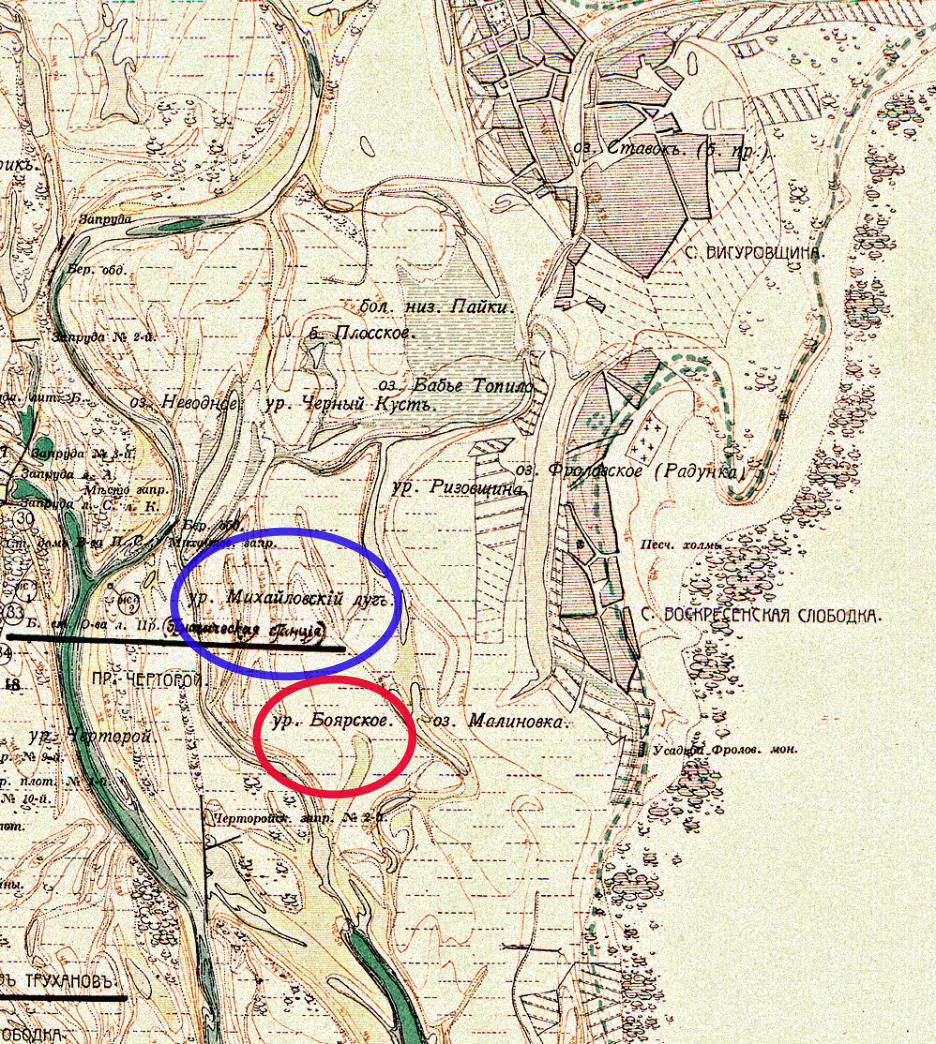
\includegraphics[width=\linewidth]{chast-gorodki/star-ist/gnil-xxx.jpg}
\end{center}

По карте 1914 года (см. выше), однако, и Малиновка, и озеро Радунка оказываются восточнее упомянутых урочищ, а не между ними, и если сопоставление сходных по именам урочищ из документа и на карте верно, то русла ни озера Радунки, ни Малиновки не считались Гнилушей.

%Я рассуждаю о местности, где русла тасовались словно карты в колоде, и сейчас от многих указанных в документах и уцелевших при этом водоемов остались только названия да примерные границы. 

%Водоемы менялись в размерах, размывались, перетекали друг в друга, соединяясь и разъединяясь, имена их не поспевали за этой текучей жизнью, тоже перетекали и путались. Хотел бы видеть мультфильм развития левобережных рек и речушек, озер, заливов и проливов, с ползущими очертаниями и названиями.  

%Даже о прошлом такой относительно крупной речки, как Радунка, можно судить урывками, понимая ее в общих чертах на большом промежутке времени, и более смутно на определенные, хотя и документированные годы. 

%Никто никогда не восстановит это в полной мере. Но смутные сгустки краеведческих сведений, постепенно собираясь один к другому, при взгляде на расстоянии дают приблизительную картину целого.

Наступил 16 век, когда частью земель в окрестностях Радунки владело семейство Викгуры или Выгуры. 

Тут выходит большая путаница. В документах 1572 года упоминается чиновник Ян Викгура, служебник Константина князя Острожского, воеводы киевского. А спустя полстолетия был такой Станислав Викгура, городничий и наместник замка Киевского. Михайловский монастырь доказывал свои права на землю тем,  что Ян Викгура был похоронен в Михайловском монастыре и завещал ему селение Викгуровщину вместе с окрестными землями.

Но вот Лидия Пономаренко в статье «Вигурівщина» (Хрещатик, 1992, 2 октября) сообщает про Станислава Викгуру, без указания года, что королевский привелей наделял его Милославщиной, однако спустя некоторое время какой-то пан Тишкович напал на селение и уничтожил его. И что Станислав Викгура на разоренном месте возродил поселение, фольварк, ставший началом собственно Выгуровщины.

Это противоречит известному про завещание Яна Викгуры, который по времени ранее Станислава уже завещал село Выгуровщину монастырю. Подлинники документов про Станислава Викгуру, пересказанных Пономаренко, я отыскать и прочесть не могу.

Весной 1654-го, Богдан Хмельницкий приказал киевскому полковнику\footnote{Полковник – правитель «полка», области. Ему подчинялись административная и судебная ветви власти в пределах «полка».} Павлу Яненку (Яновичу) привести в исполнение передачу Выгуровщины Михайловскому монастырю, в лице игумена Феодосия Василевича\cite[82]{mihdocs}:

\begin{quotation}
Той же Богдан, гетман, киевскому полковникови о надани Викгуровщины монастиреви Золотоверхому обявляет, препятствователей же владиния монастирскому и обывателей без пощадиния повеливает наказовати.

Богдан Хмелницкий, гетман з Войском его црского пресвитлого величества Запорозким.

Пне полковнику киевский.

А иж подалисте Викгуровщину зо всими пожитками и приналежностями, до оное належачими, его млсти отцу Василиевичу, архимандрити слуцкому, игуменови монастира Михайловского, на монастир михайловский, прето жадаем вас и напоминаем, жебы его млсти отцу архимандрити в той Викгуровщини перешкоди не було, але абы вцеле вшелякие пожитки доходили и жаден жебы кгрунтов тамошних и сеножат не займовал, а кгди которий бы перешкоду чинил, такового в. мст срокго карай.\\

При том в. м. Гсду Бгу поручаем.

Дат з Чегирина, дня 21 мая 1654.

Богдан Хмелницкий, рука власная.
\end{quotation}

Гетман также универсалом поставил жителей Выгуровщины, кроме казаков, монастырю в подданство\cite[81]{mihdocs}: 

\begin{quotation}
Той же Богдан, гетман, мистечко Викгуровщину со обстоятелстви и мищанским послушанием всяким и показанщиною от винокурен козацких без всякого их противления монастиреви Михайловскому отдает универсалом.

Богдан Хмелницкий, гетман з Войском его црского пресвитлого величества Запорозким.

Ознаймуем сим ншим писанием, кому бы о том видат надлежало, меновите пну полковникови киевскому, также козаком и мещаном мистечка Викгуровщини обывателем, иж ми тое мистечко Викгуровщизну з ставами, синожатми, озерами, полями и иншими всими акциденциями, которих перед войною дедичнии пнове и их намисники заживали з арендами вшелякими так пивними, яко медовими и горилчаними, конферовали на монастир стого архистратига Михаила Золотоверхого.

Зачим мити хочем и владзею ншею приказуем, абысте вси, котории одно до повинностей миских належите и не естесте козаками, вшелякое послушенство и подданство его млсти отцу Феодосию Василиевичуа, архимандрите слуцкому а игуменови монастира тамошнего михайловского, также намисникови его, там зосланому, отдавали; козаки жебы в жаднии найменшие провента не втручалис, ани жадними шинками не бавилис под строкгим войсковим каранем, показанщизну абы вси звичайне, як и всюди так козаки, як и мещане, кром жадного спротивленя се отдавали, не чинечи иначей; а котории би якую колвек чинили кривду и
перешкоду, так козаки, яко и мещане, ежели бы не послушними были, таковий кождий сурового войскового не уйдет караня.\\

Дат з Чигирина, дня 22 мая, року 1654.\\
Богдан Хмелницкий, рука власная.
\end{quotation}

Но местные сопротивлялись этому решению вплоть до семидесятых годов того же века, а земельные споры, как увидим далее, продолжались еще столетиями.

Во время ближайшее к смерти Станислава Выкгуры, на угодия доказывали права Троицкий Больничный монастырь, священник киевской Воскресенской церкви Кирило Муха (не зря же Воскресенская слободка поблизости от Выгуровщины и Троещины), да служилый человек Быримович. А у Михайловского монастыря, по словам его представителей, не осталось никаких документов на эти земли – всё увезли с собой Поляки при смене власти.

%В 1657 году в селе Выгуровщина киевский полковник Василий Дворецкий, обмерив границы, издал приказ, изложив в нем суть дела и собственно границы Выкгуровских владений\footnote{Документ даю по статье Мицик, Ю. Документ до історії Вігурівщини: [з історії місцевості] // Київська старовина, 1994, №5. с. 71-73.}. Привожу документ целиком. Отметим, что граница уже не от Днепра, а сразу от Радунки, и в помине нет Милославщины – ее заменила собой Выкгуровщина.

В 1657 году в селе Выгуровщина киевский полковник Василий Дворецкий, обмерив границы, издал приказ, изложив в нем суть дела и собственно границы Выкгуровских владений. Привожу документ целиком\cite{mihdocs}. Отметим, что граница уже не от Днепра, а сразу от Радунки, и в помине нет Милославщины – ее заменила собой Выкгуровщина.

\begin{quotation}
Василий Дворецкий, полковник Войска его царского пресвитлого величества Запорозский наказный киевский.

Ведомо чиним тим писанем нашим всим вобец и кожному зособна, кому б о том видат тепер и в потомные часы належало, а меновите старшини и черни козаком Войска его царского пресвитлого величества Запорозского и кождой кондиции на урядах и Киеве людом и посполитим мешканцам по селах и хуторах около Киева мешкаючим, до видомости доносим, иж з виразной воли и росказаня его милости пана Богдана Хмелницкого, гетмана Войска его царского пресвитлого величества Запорозского, и з росказаня пана Павла Яновича Хмелницкого, полковника своего киевского, выежджалисмо до села Викгуровщины, монастиру святому Михайлу Золотоверхому на выживене взглядом великого знищеня помененого монастиря даной\footnote{Выехали в село Викгуровщину, которое дано монастырю Михайловскому Златоверхому в прокормление (выживене) по случаю большого обнищания (знищення) упомянутого монастыря.} и для того, же тот Викгура, которий Викгуровщину осаждал и держал\footnote{Создал, населил и владел ею.}, по смерти своей положен ест в том же монастиру Михайловском из тых причин тое селце Викгуровщину с то милость пан Богдан Хмелницкий, гетман Войска Запорозского, на поменений монастир надал, а же отца игумена и всю братию монастира Михайловского почали были о кгрунт Викгуровский турбоват\footnote{Игумена и братию Михайловского монастыря, по поводу земли Викгуровской начали беспокоить такие-то.} з едной стороны отцеве троецкие, з другой – отец Кирило Муха, священник Воскресенский киевский з свойми парохиянами и ктиторами о отчину воскресенскую, о чом и до его милости пана гетмана удавалися; з третего боку – Биримович, служащий человик, маючий соби частку купленого кгрунту; и той помененый кгрунт Викгуровский на части хотячи розервати.

А кды там же перед нами, от превелебного отца Феодосия Софоновича, игумена монастыра Михайловского отец намистник Сергий з братиею своею засланый был, отцеве троецкие и священник воскресенский с парохианами и Быримович, яко стороны поводовие станули, указовали розные листи, отец намистник з братиею своею, не могучи прав страчоных того села показати, же ляхи права в Полщу з собою позавозили, одно наданые его милости пана гетмана указуючи, мужей старинных и добре того кгрунту свидомых, болшей десяти на свидецтво ставили, которие от нас питани были под сумненем\footnote{«Под сумненем» – письменное показание с росписью свидетеля. Пример: «водлуг права духовного свядецтвом устным и под сумененм доводили».} признали, иж з давных виков тое селце никгди никому иншому не належало, тылко небожчикови Викгури\footnote{Старожилы свидетельствовали на местности, где какие урочища находятся, и что Викгуровщина и земли ея никому, кроме покойника Викгуры, не принадлежали.}, на которое, мовят, мы свидоми, же он и права от королей полских мил и нам указовал и граница з вику того селца такою ест:

1. Почавши от рики Радонки на конец поповой синожати подле Троеччины до озерца, що над чорториею,

2. от озерца долиною ку старому кладовищу вправо – кгрунт Викгуровский, а вливо – троецкий, идучи ку городищу прежднему подле борку, где замочок и двор был князя Семена Олелковича,

3. а от городища, также подле борку, на поле прудец, 

4. прудцем до трох курганов, 

5. от курганов на конец кривой нивы мимо селище до рички Угнору,

6. Угнором вгору идучи, вправо кгрунт Викгуровский Березовичи, а вливо троецкий до болота Куричова,

7. через Куричово, подле кривого дуба на перевис до сторожевых гор, где сосны значены крестами, 

8. от Сторожевых гор долиною через озеро Ковпит до болота Облуквы и до Чорной Воды, 

9. от Чорной Воды долиною до шляху Басанского, тым шляхом Басанским идучи ку Киеву вправо кгрунт Викгуровский, а вливо – николский, аж до шляху, идучого з Бровар до Викгуровщины. 

10. Тим шляхом повернувши, вправо – кгрунт Викгуровский, а вливо – воскресенский, мимо криницы аж до Писчаних гор\footnote{Левобережная Лысая гора?},

11. Писчаными горами до болота Корчовки, Корчовкою до рубежа ровчака, текучого з озера Мокрицкого,

12. тим рубежом в Гнилушу, ричку; 

13. Гнилушою мимо Викгуровщины опят до рички Радонки\footnote{Несколько другой вариант «ограничивания» приведен как выдержка из описи владений Михайловского монастыря, опубликованной в «Приложениях к хронике К. Михайловского монастыря» в томе «Прибавлений» к «Киевским епархиальным ведомостям» за 1861 год:

1. почавши от речки Радунки на конец поповой сеножати подле Троечцини до озера що над Чорториею;

2. от озерца долиною к старому кладовищу, в право грунт вигуровский, в лево троецкий идучи ко городищу прежнему подле Борка, где замочок и двор был князя Семена Олелковича; 

3. а от городища тамже подле Борку на поле Прудец; 

4. Прудцем до трех курганов,

5. на конец кривой нивы мимо селище до речки Угнору;

6. Угнором в гору идучи, в право грунт Вигуровский Березовица, а в лево Троецкий до болота Куречового;

7. через Куречово подле кривого дуба на перевес до сторожовых гор, где озеро Ковпыт, до болота Обловки и до чорной воды;

8. от чорной воды долиною до шляху Басанского; тим шляхом Басанским идучи до Киеву в право грунт Вигуровский, а в лево Никольский, аж до шляху идучого з Бровар до Вегуровщины;

9. тим шляхом повернувшися до Вегуровщины в право грунт Вигуровский, а в лево Воскресенский, мимо криницы аж до Песчаных гор;

10. тыми пещаными горами до болота Корчовки;

11. Корчовкою до Рубижа ровчака, текучого з озера Мокрицкого;

12. тим Рубижем в Гнилушу речку;

13. Гнилушею в гору мимо Вигуровщину и паки до речки Радунки.}.

Где мы пилно то выслухавши, и сами, яко з молодых лит у Киеве живучи и почасти свидоми, ани на троецком кгрунту, ани на Воскресенском, aни на Быримончовом тое селцо Викгуровка, але на королевском, от королей Викгуре надана ест и осажена, теды монастыреви святому Михайловскому Златоверхому киевскому вичне присудилисмо\footnote{Сам полковник Дворецкий выступает здесь в роли старожила, свидетельствуя в пользу принадлежности земли Викгуровки поначалу королю, а затем жалованной им Викгуре, и после – монастырю Михайловскому.}, абы ведлуг\footnote{В\'едлуг – в силу.} наданю\footnote{Наданя – жалование, грамота в подтверждение прав на землевладение.} его милости пана гетмана, яко перед тым и в далший час тое селцо Викгуровщину отец игумен михайловский з братиею своею спокойне держал и пожитки вшелякие уживал, ижебы отцене троецкие, ани парохиане воскресенские\footnote{Парафиане, прихожане Воскресенской церкви. «Парафия» это искаженное греческое «παροικία» («пароикия»), буквально «возле дома», а так – «приход».}, ани Быримович того села и его кгрунту болшей турбации\footnote{Беспокойства.} отцу игумену св. михайловскому не чинили и его братии, а селяне викгуровские, абы отцу игуменови свято-михайловскому и от его высланым вшелякое послушенство отдавали и повинност свою полнили\footnote{Проще говоря, чтобы селяне исправно платили налоги игумену Михайловского монастыря либо его представителям.}, козаки абы ниякой перешкоди не чинили\footnote{А местные же казаки (особое сословие, не крестьяне) тому не препятствовали.} и ведлуг универсалу его милости пана гетмана заховалися на що для болшой вири и твердости в той справе висланым будучи до того писаня нашого руками нашими подписавшися, печати притиснувши отцу игуменови монастыра свято-михайловского Златоверхого киевского и братии его даемо.

Диялося в силци Викгуровщини июля 2 дня 1657 року. Филипп Стефанович Скороход, писар полку киевского высланый Звышленований, рукою власною.

От Петра Бутрима, атамана городового киевского в той же справе высланый, яко писат неумиючого, писар его подписуюся Матвий Зубикович, рукою (власаною)
\end{quotation}

Порассуждаем над каждым из пронумерованных «шагов».

1. Речка Радунка соседствовала с поповой сеножатью около Троещины. Там было и озеро «над Черторыей» – возможно Троицкое, что лежало севернее Троещины.

Однако любопытно, что «над» это ведь к северу. Но если бы река Черторыя текла от Десны, то над Черторыей может быть только Десна, а не озеро. Следовательно, Черторыей в документе называется русло, подходящее к широте, условно говоря, Троещины, откуда-то сбоку, например с запада. От Днепра наискось через Муромец. Только так обеспечивается условие «над». Значит, прежде Днепр пробился к левому берегу севернее известного места между Московским и Петровским мостами. И позже в тот рукав Днепра сверху пробилась Десна.

2. От сего озерца – «долиною к старому кладовищу» – вероятно на юг или восток, ведь по ходу направо будут земли Вигуровские, налево – Троицкие. Сохраняя направление, мы дойдем к «городищу прежнему подле Борка, где замочок и двор был князя Семена Олелковича».

3. «а от городища тамже подле Борку на поле Прудец». Прудец расположен на поле, или Прудец это название поля? На картах есть водоем Прудок или – на карте лоций 1914 года – «Ставок», но «ставка» нет в земельных документах, может это перевод составителя карты лоций.

4, 5. Этим Прудком можно было добраться до трех курганов, в конец «кривой нивы» мимо «селища» и до речки Угнора. Селищем именовали заброшенное село, как «городище» – былой город, «замковище» – былой замок.

6. Двигаясь по Угнору на север, вправо будет Березовица, владение Вигуровское, а влево – земля Троицкого монастыря. Так граница идет «до болота Куричового», причем это определение относится не к земле Троицкого монастыря, мол, она простирается до болота, но относится именно ко границе, поскольку пункт шестой гласит «через Куречово подле кривого дуба на перевес до сторожовых гор, где озеро Ковпыт, до болота Обловки и до чорной воды». Итак, Угнором граница длится до болота Куричового, и по нему, возле Кривого дуба, на перевес.

Болото Куричево, поскольку туда идет граница по Угнору, сопоставляю с болотом, которое потом стало Алмазным озером. На современных картах урочищем Куричевым иногда подписывают Большую поляну – полагаю ошибочно. Из болота, прежде заполнявшего поляну и окрестности, никакой Угнор вытекать на запад к Выгуровщине не мог, ибо западный берег был и остается горой. Течь вода к Выгуровщине, по рельефу, могла только от нынешнего Алмазного.

7. «Перевес» означает застава. Между Куричевым около кривого дуба был перевес на Сторожевые горы, а от них граница шла к озеру Ковпыт.

Ковпыт ныне – осушенное в северной и южной своих частях болото, где в 20 веке добывали торф. В 1634 году на одноименном озере, принадлежавшему Михайловскому монастырю, стояла мельница, а значит, протекал ручей, и при нем была плотина. Так вот почему заболотилось озеро! Вспомним судьбу реки Дарницы и цепи болот, на которые она распалась на большом протяжении. 

Озеро, затем болото Ковпыт раньше тянулось от широты Погребов до широты Выгуровщины, параллельно Куричеву, восточнее, отделенное от него – выходит, Сторожевыми горами. Вот вам и название горбов, на которых стоит ТЭЦ-6 и что составляют восточный берег Алмазного озера. Тот самый высокий берег прежнего русла Десны.

8. «Черная вода» – возможно, связь с торфяным болотом. Про Басанский шлях я ничего не скажу, кроме того, что к востоку от Броваров есть речка Басань, а на ней село Старая Басань. От этого шляха граница шла к другому, дороге от Броваров до Выгуровщины. Он хорошо виден на карте 19 века Шуберта, проходя по лесу южнее «болота Колпытского».

9, 10 – «песчаные горы» – полагаю, цепь дюн Лысой горы, идущая вдоль Воскресенки и по ней к болоту Корчовке.

11. Ровчак «рубиж» или «рубеж». Ровчак это пробитое водой небольшое русло либо канал. Мокрицкое озеро теперь называют Радункой. «Рубежом» в старину называли межу, границу. Ровчак и служит границей.

Красным я подчеркнул «рубеж» на карте Шуберта – от верховья озера Радунки он, задав начало Малиновки (у Шуберта не обозначена), проходил до Неводного. Помните про разницу в столетиях между описанием границы и картой!

\begin{center}
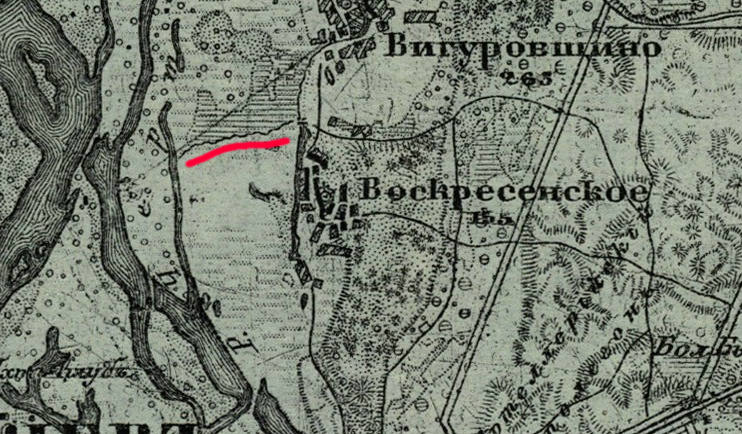
\includegraphics[width=\linewidth]{chast-gorodki/star-ist/rubij.jpg}
\end{center}

12, 13. Ровчак-рубеж впадал в речку Гнилушу, а Гнилушей мимо Выгуровщины мы достигаем речки Радунки. Обе речки указаны раздельно. 

В уточнении ровчака-рубежа поможет другая выдержка из описей владений Михайловского монастыря. К сожалению, в публикации «Епархиальных ведомостей» не указаны годы.

Читаем следующее о некотором земельном владении:

\begin{quotation}
В ограничении таком лежачий: почавший от головы озера Мокрицкого долиной подле футора черниц Флоровских в лево грунт флоровский, а в право михайловский до футора Ризичиного належачий, тоею долиною в речку Меленовку; Меленовкою в Гнилушу речку, Гнилушею в гору до Рубежа ровчака, Рубежем в гору до вершины знову озера Мокрицкого.
\end{quotation}

Озеро Мокрицкое это нынешнее Радунка около Воскресенки. А что за речка Меленовка? Очевидно, современное озеро Малиновка, параллельное озеру Радунке, это речка Меленовка либо ее часть. И написано даже, что Рубеж – около вершины Мокрицкого (озера Радунки). Так и есть.

Некоторую путаницу вносит написание «Рубежа» с большой буквы в ряде документов – можно подумать, что это собственное имя водоема, но, как покажу дальше, это ошибка.

Упомянутый же ровчак-рубиж возле Воскресенки, как я понимаю из документов, соединялся со следующими водоемами – озером Радункой (Мокрицким), Меленовкой и речкой Гнилушей. Русло последней около Воскресенки я покамест не могу вычислить.

Окрестности Воскресенки, однако не она сама (Воскресенская церковь, что на Подоле, лишилась этого имения в 1719 году, а к концу того же века слободка стала казенной), издавна были владением Флоровского монастыря. Даже озеро Радунка на карте лоций 1914 года подписано: «оз. Фроловское (Радунка)». Там же находим бывший хутор Ризичин или Ризивщовну – «урочище Ризовщину», чье название свидетельствует о прошлом. Ризовщина находилась между озерами Радункой и Малиновкой, там теперь Воскресенские сады.

Универсал Мазепы освобождал волошских поселенцев на этом хуторе от войсковых податей\cite[96]{mihdocs}: 

\begin{quotation}
Гетман той же Мазепа людей волоских на земли монастирской на хутори Ризивщовни во окрестности Викгуровской ново осажених оборонним универсалом от податей войскових уволняет.

Их царского пресвитлого величества Войска Запорозского гетман Иван Мазепа.

Ознаймуем сим ншим универсалом кождому, кому о том видати належит, а особливе пну полковнику киевскому, сотникови тамошному, также войтови зо всими маистратовими тамошними, иж донесл нам превелебний в Бгу гспдн отец Силвестр Головчич, игумен михайловский киевский, же купил он част земли близко маетности монастира своего села Викгуровщини, на которой части земли осадив килка члвка волоских людей и просил нас, абисмо уволнили тих его людей от подачок и всяких войскових повинностей.

Теди ми, гетман, принявши тое его отца игуменово прошение, даем ему сей наш оборонний универсал, через которий мити хочем и приказуем, абы нихто з старшини и черни не важился потягати тих его волоских людей до войскових подачок и до жадних повинностей.

Дан в Батурини июля 31 д. року 1694.

Звишменованний гетман, рукою власною.
\end{quotation}

Но вернемся к Выгуровщине. 

Гошкевич в статье тоже приводит «ограничение» Дворецкого, лишенное вступления с сутью дела и окончания – просто саму опись. И она отличается от помещенного мною ограничения. Нет упоминания про Басанский шлях, вместо озера «Ковпыт» написано «Ковтир», а болото «Обловка» – «Облоква».

Гошкевич опубликовал также выдержку из некоего, как он говорит, древнего акта границ села Троещины, данную Троицкому Больничному монастырю в 1719 году киевской губернской канцелярией в связи с тем, что бумаги по землевладению сгорели в Лавре во время пожара 21 апреля 1718 года. Но это границы не только деревни Троещины, однако и смежных с ней прочих угодий Троицкого монастыря. За какое время? Положим хотя бы 17 век или самое начало 18-го. Я позволил себе заменить некоторые слова – некоторые «да» на «до», а также отделить слитное написание предлогов.

\begin{quotation}
Граница которая починается от 

1. Днепра старым деснищем у днеприще старое сухое

2. а днеприщем сухим у озеро бобровню 

3. з бобровни стариком у озеро которое называетца теперь речищем 

4. а с речища през радунку речку к старому кладовищу 

5. от кладовища подля борку – в городище, где был двор князя Семиона Олелковича

6. там же у речку прудец

7. а прудцем в гору живцем до стойла татарского

8. а от стойла татарского гнором до кривой нивы

9. да гнором до осинового леса поуз той же гнор до краснаго дуба

10. оттол гнором до овдютины дубровы

11. от дубровы гнором поуз шипилков рог да у речку рубеж

12. тем рубежом до терна

13. да поуз вечи речкою рубежем у речку кодачок что идет к погребом

14. а тою речкую вгору да и в десну

15. а десною вниз в старое деснище

16. да поуз мардасов к острову Марковы Головы

17. от того урочища до сопля сухим деснищем у возверницу 

18. мимо речку келнища до старого деснища откуда почалися грани.
\end{quotation}

Разберем некоторые шаги. Помним, что границы владений Троицкого монастыря частично соседствуют с границами Михайловского, например, как понимаю, по Прудцу в одну сторону лежат владения одного, по иную – другого.

Снова кстати особенность – ни слова нет о Черторые. Стало быть, на время составления документа, Черторыей считался водоем южнее описываемой местности, однако позже название Черторыи распространилось и севернее, на какое-то из русел, проходящих по острову Муромцу от Днепра на восток. Все эти днеприща и речища, следы прорывов Днепра.

Первые три шага проясняются с большим трудом, поскольку затрагивают местность, которая сильно изменилась.
 
1, 2. Граница начинается у Днепра, на западном берегу земель, известных ныне как остров Муромец, в северной его части. На время документа это был, полагаю, не остров, а еще материк. «Старое деснище» – некий рукав Десны, старое его русло, а «Старое днеприще сухое» – обмелевший рукав Днепра. По нему граница переходит на восток к озеру Бобровне. На карте лоций 1914 года Бобровня – урочище чуть южнее обоих озер Кинищ.

3. Из Бобровни стариком в озеро Речище. Под речищем мне видится нынешнее озеро Старая Речка, что огибает Калиновку.

4. «А с речища през радунку речку к старому кладовищу». От Речища через Радунку речку к старому кладовищу. Кладбище – рядом с борком, борок – чуть севернее Выгуровщины и южнее Троещины. 

%Поскольку Черторыя тут не упомянута, очевидно, что ее на этой широте нет.

5. От кладбища около борка граница тянулась в городище, где был «двор Семиона Олелковича». Всё около борка – кладбище и городище.

6. «У речку Прудец» – свидетельствует о текучести воды в Прудке.

Далее подробно обсуждать шаги описи я не решаюсь, сделаю несколько замечаний. Живец – ручей, то бишь по Прудку, ручьем граница шла до Стойла Татарского. Быть может память, что там останавливался Меньгукан?% Видно ли оттуда было Киев? 

Шаги 13, 14 – «да поуз вечи\footnote{Вечи – ветлы, вербы?} речкою рубежем у речку кодачок что идет к погребом» и «а тою речкою вгору да и в десну» противоречивы.

Ранее мы встречали ровчак-рубеж – длинное русло между озерами Радункой, Малиновкой и Неводным, по верховьям первых, и на запад оттуда Кодачок – ныне урочище Горбачиха около Русановских садов.

Однако возле Погребов была своя речка Кодачок и урочище Закодачче.

Вероятно, слово «кодачок» и «кодак» что-то означало и применялось к разным водоемам. У днепровских порогов была крепость Кодак, и  наука полагает, что в переводе с тюркского это слово означает «поселение на горе», однако простейший просмотр карты Украины показывает, что существует много селений с названием Кодак, Кодачок, всегда при какой-то речке. Похилевич в «Сказаниях» толкует с татарского слово «койдак»  как лес. Думаю, можно сыскать и водный перевод – знать бы с какого языка. 

С речкой Кодачок (что около Погребов) связана речка-рубеж – другой водоем, не тот, что протекал близ Воскресенской слободки.

Я не знаю, где именно был этот «погребской» Кодачок. Может так называлось русло, что было рукавом Десны к востоку от современной Десенки и впадало в нее около «старой» Троещины? Или со стороны Погребов когда-то шел еще один рукав Десны?

%Но в Рубеже и Кодачке я уверен по земельной описи, где упомянута Воскресенская слободка Флоровского монастыря.

Шаг 16-й: «да поуз мардасов к острову Марковы Головы» – на лоции 1914 года отмечены озера Марковица и Мордосов, очевидно то же самое. Они лежали на северном берегу Десны, первое примерно выше истока современной Черторыи, а второе на северо-восток от устья Десны, точно соотнести не берусь. Остров же Марковы Головы мы наверняка можем связать с озером Марковицей, и тогда выходит, что это полуостров точно напротив начала Десенки, огибаемый резкой полупетлей Десны.

Наконец, шаг 18 – «мимо речку келнища до старого деснища откуда почалися грани». Келнище это нынешнее озеро Кинище и, вероятно, близкое к нему на юго-восток Малое Кинище, оно же Подкова. 

На рубеже 17-18 веков Михайловский монастырь много скупил владений у независимых и относительно мелких землевладельцев – казаков Выгуровщины. «Пляцы» (участки с постройками), и «грунты» (участки земельные). Сохранились купчие. В документе 1700 года всплывают названия урочищ Стуйло «над болотом Корчувкою» (то самое Стойло Татарское?), Березовица, что «за городищем», ближние и дальние Будищи, «городищи», болото Корчовка. Полезно прочесть, заодно чтобы знать, что сколько стоило\cite{mihdocs}:

\begin{quotation}
Ми, нижей на подписи вираженные, чиним видомо и признаемо сим писанием нашим, кому би тепер и на потомные часи видати належало, иж ми, будучи здоровими на тили и на умисли, продалисмо доброволне грунта наши козацкие в сели Вигуровщини, до манастира Михайловского Золотоверхаго киевского, превелебному в Бгу его млсти господину отцу Силвестру Головчичу, игумену монастира тогож. 

Я, Андрей Козак, мелник вигуровский, продал двор з пляцом в сели Вигуровщини со всими грунтами своими власними, належитими на Стуйли, на Березовици за городищем, и где едно вси знайдуются грунта орание и неорание, зарослие и синожати и со всяким угодием за золотих осмъдесят в року тисяча шестъсотним девятьдесят пятом, мсца мая пятого дня за атаманства Яска Перехриста старого.

Я, Феодор Мосиенко, тому ж отцу Головчичу, игумену монастира Михайловского, продалем двор в сели Вигуровщини и поля ближные будища, три ниви прилеглие грунтам монастирским на Cтуйли, за городищами дви ныви, на Березовци также три ниви, и где одно грунта знайдуются орание и неорание, зарослие синожати и со всяким угодием, за золотих седмдесят три в року тисяча шестьсот девятдесять семом мсця февруариа девятого дня, за атаманства Феодора Перехристенка.

Я, Иван Чичиль, тому ж превелебному в Бгу отцу Головчичу, игумену монастира Михайловского, продал двор в сели Вигуровщини з нивами и грунтами на Березовици ныв чотири, за городищами нива великая, которая в лан монастиръский вораная: так теж и три нивки менших на Стуйли, нива великая в рогу над болотом Корчовкою и дви ниви менших на Стуйли пятьдесят пять в року тися шестьсот девятьдесять семом, мсця марта пятого дня, за атаманства Никиты Тарана.

Року тисяча шесть соть девятьдесят осмого, мсца февруария двадцять пятого дня, по смерти небожка отца игумена монастира Михайловского киевского, теперешному отцу Захарии Корниловичу, игумену того ж монастира Золотоверхого киевского продал я, Феодор Перехристенко, двор з пляцом, з грунтами и со всими до их приналежностями за золотих тридцять пять.

Року того ж, мсця марта осмнадцятого дня, продал я, Никита Таран, ниви дви великие в далших Будищах, прилеглие ланам монастирским и за городищем так же нив дви за золотих сорок.

Року того ж, мсця мая шестого дня, продал я, Иван Дрозденко, тому ж отцу игуменови ниви в Куричеви, ниву великую в Будищах, ниву великую обмеж монастирских нив, на Березовици нив дви, за городищами една, и поля зарослие и синожати за золотих сорок пять.

Року того ж, мсця мая осмнацятого дня, продал я, Вакула Опанасенко, козак вигуровский на Березовци ниву великую, обмежу монастирской ниви и менших нивок дви, за городищем нив дви, на Стуйли нива една, у Будищах нив дви и вси поля орание и синожати за золотих тридцять три. 

Року того ж, мсця юня четвертого дня, продал я, Грицко Коломиец, на Березовци нив дви, за городищами нив дви, у Будищах една, на Стуйли три нивки за золотих пятнадцять.

Року того ж, мсця юня пятнацятого дня, продала я, Одарочка, вдовиця, двор з пляцом, з грунтами и зо всими до того двора приналежитостями за золотых пятнадцать.

Року того ж, мсця юля двадцять семого дня, продал я Ияков Перехрестенко, атаман вигуровский, ниву великую за городищем вораную в лан монастирський, за золотих сорок.

На что мы вси, сполне соединившися з тоей продажи, сим писмом зрекаемся так самим, яко и потомком нашим вичними часи жадного приступу
и вмищатися в тые грунта не зоставуючи.

Упросилисмо для липшой певности в потомные часы людей вири годних и подпис рук.

Диялося в сели Вигуровщини. Року тисяча седмсотнем мисяця септемврия осмого.

Яков Прехристенко, атаман вигуровский.

Я, Хведор Перехристеко

+ Иван Дрозд

+ Павел Тараненко

+ Грицко Коломиец

+ Одарочка Василиха

+ Вакула Опанасенко

+ По смерти тестя своего Иван Олексиевич Доромирецкий
\end{quotation}

В 1704 году киевский митрополит Варлаам Ясинский назначил комиссию для решения земельного спора между Троицким и Михайловским монастырями. Протокол ее работы всплывает десять лет спустя, 27 июля 1714 года, в декрете из книг Генерального военного суда про размежевание Викгуровских и Троещинских грунтов в судебной тяжбе между Свято-Троицким Больничным и Свято-Михайловском Златоверхим монастырями.

С этим поучительным документом тоже познакомимся в полном объеме, дабы получить представление, как тогда решались земельные споры, и как легко урочища переменяли свои положения согласно показанию свидетелей-старожилов и вмешательству заинтересованных сторон.

\begin{quotation}
Року тисяча семсот чотирнадцятого, мсця июля двадцять семого дня. За видомом его царского прсвитлого величества Войска Запорожского обоих сторон Днепра гетмана ясне велможного его милости пана Иоанна Скоропадского перед судом его царского прсвитлого величества Войска
Запорожского енералным было право законников мнастира Сто-Михайловс\-кого Золотоверхого киевского о розграниченю кгрунтов презентованное, которое ку вечистому записаню, як ся оное в себи мает до книг судовых принятое в такый текст:\\

Року Бжого тисяча семсот четвертого мсця июля двадцат четвертого.

До рук ясне в Бгу преосвщенного его милости отца кир Варлаама Ясинского Бжиею милостию православного архиепспа метрополита киевского, галицкого и всея России, подали супплику законники монастира Сто-Михайловс\-кого Золотоверхого киевского, жалостно у скар\-жаючися на превелебного отца Евстратия Чудикевича, игумена мнастира сто-Троецкого Болницкого заворотного Киево-Печерско\-го, в той способ, иж оны, законники сто-Михайловские, маючи от славной памяти гетмана п. Богдана Хмелницкого по небожчику пану Яну Викгури, в том же Михайловском мнастири погребенном, село Викгуровщину для виживленя за небожчика отца Феодосия Софоновича, игумена михайловского ж року 1654 наданное, а року 1657, по указу того ж славной памяти гетмана п. Богдана Хмелницкого и по росказаню п. Павла Яновича Хмельницкого, полковника киевского, киевским же полковником наказним п. Василием Дворецким при притомности людей з трох сторон многонародной, на он час доводне ограниченние, а сими часы превелебный отец игумен свято-троецкий з поддаными троецкими на их кгрунту викгуровском оседаючими, много кгрунтов викгуровских около борка в правой руце неведать яким правом отбирает, надто еще вдирается аж по самое городище старое князя Семена Олелковича.
\end{quotation}

Законники (юристы) Свято-Михайловского Златоверхого монастыря подали суплику (прошение, жалоба, от латинского suplices literae) Варлааму Ясинскому, православному архиепискому метрополиту киевскому, галицкому и всея России, на  преподобного отца Евстратия Чудикевича, игумена монастыра Свято-Троецкого Болницкого.

Законники утверждали, что монастырь их Михайловский владеет, от покойного Яна Викгуры, в том же монастыре погребенном, селом Викгуровщиной, отписанной монастырю при покойном игумене Феодосии Софоновиче в 1654 году. В 1657 указом Хмельницкого было проведено полковником Василием Дворецким ограничение, то бишь размежевание. Но в последнее время преподобный отец игумен свято-троецкий со своими подданными, осевшими на викгуровской земле, невесть по какому праву прибрали к своим рукам много викгуровских участков по правую руку от борка, добравшись «аж по самое старое городище князя Семена Олелковича».

Слово «право», если не про руку, здесь имеет определенное значение – разумеются документы, в которых подтверждается владение участком земли и прописаны его границы.
 
\begin{quotation}
На якое поле месяца июля числа 21 в пятницу против субботы вночи, важился отец игумен святотроецкий насподевание наслати людей служалих броварских и забрати пожатого жита на сто коп, а стоячого на пни, возами и конми шкодливе потратовати.

Что послушник свято-михайловский городничий викгуровский иеромонах Иакинф послишавши, кгды в поле виехал боронити того жита, теды и того городничого на кони сидячого поймавши, и держачи за руки тие насланники игуменские нещадно побили киями, по голове, по пличах, по руках, в великим увеччем здоровя, мало аж не ку смерти, когда бы без клубука и подкапиа зрозшарпаною рясою не умкнул до викгуровщины за оброного людей тамошных.
\end{quotation} 

21 июля, в ночь с пятницы на субботу, игумен «насподевание» (внезапно) прислал на поле, служащее предметом разбираемого ныне земельного спора, «людей служалих броварских»\footnote{Бровары, городок под Киевом, издавна принадлежал Троицкому Больничному монастырю Киево-Печерской Лавры, а по некоторым данным был им же основан в 1593 году.}, которые забрали на сто коп\footnote{Копой применительно к урожаю считалось 60 снопов. Копой именовали также 50 литовских копеек серебром.} сжатого жита\footnote{Житом называли то просто хлеб, то именно рожь.}, а несжатое («стоячого») потоптали возами и конями. 

Выехав в поле на коне, послушник Михайловского монастыря, городничий викгуровский, иеромонах Иакинф пытался помешать увозу жита. Его поймали и, держа за руки, беспощадно побили киями (палками) по голове, рукам, плечам – изувечили почти до смерти, если б не вырвался и в разорванной рясе не убежал в Викгуровщину под защиту тамошних людей.

\begin{quotation}
а любо велебный отц Никифор, намисник сто-Ми\-хайловский, завчасу забигаючи такому зуфалству, избил до отца игумена троецкого з своими правами и крипостми вишше именованими, просячи, жебы не велил своих перехвалок виконивати, леч абы, албо полюбовне рачил обийтися, албо правне з нами поступити, есми ему якая диется кривда, еднак отц игумен сто-троецкий и приобицавши свою любов и спокойност, важился самоволне несподиванную мнастиреви Михайловскому вышше описанную учинити обиду и укоризну. 
\end{quotation}

За какое-то время до этого, отец Никифор, наместник Свято-Михайловского монастыря, отбыл к игумену Троецкому со своими «правами и крепостями» – документами на землевладение – вышеупомянутыми (имеется в виду ограничение Дворецкого и так далее), надеясь решить дело про спорный участок полюбовно, однако святотроицкий игумен, пообещав в этом деле «свою любов и спокойност», осмелился самовольно нанести Михайловскому монастырю неожиданную обиду, описанную выше.

\begin{quotation}
А при той суплици Клым Бутенко и Марко
Куриленко, козаки старожитние выкгуровские, подавали суплику, жалуючися в той способ, иж и оныи отци их еще за Выкгуры небожчика свободне свои поля за городищем порожным Олелковым орували, сивали и збирали, ны от кого не збороные. А тепер отц игумен сто-троецкий, наславши своих людей служалих броварских, забрали им в копах жито, а гречку, просо и остаток жита на пни внивец потолочили и возами, и конми потратовали. 
\end{quotation}

При той жалобе, поданной законниками михайловскими митрополиту, выгуровские казаки- старожилы, тоже подали суплику по тому же поводу, что отцы их еще при Выкгуре свободно на своих полях за пустым городищем Олелковым пахали, сеяли и собирали урожай, и никем это не воспрещалось. А теперь отец игумен святотроицкий, наслал людей служилых броварских, они забрали у козаков сжатое жито, а гречку, просо и остатки жита потравили конями и возами.

\begin{quotation}
Где просили преосвященного пастра его милости, жебы албо вложился за ними, до кого належит, албо жебы им позволил ехати з челобитною до ясне велможного добродия его милости пна гетмана в войско, кгдыж там синове их горлуют, а оны, яко господари, зоставшися для зобраня пашенки своей при великой утрати праци своей насиловани зостали невиные. 
\end{quotation}

В жалобе, козаки просили митрополита, чтобы или разобрался сам, кому земля принадлежит, или позволил им ехать с челобитной к ясновельможному пану гетману в войско, где служат их сыновья, а они (козаки, подавшие жалобу), как хозяева, оставшиеся для сбора урожая, невинно пострадали и понесли большие убытки.

\begin{quotation}
Тие обидви суплики ясне в Бгу преосщеный пастир его милост милостивно принявши, посилал до ясне в Бгу превелебного его милости отца Иоасафа Кроковского, архимандрита свтой Лавры Киево-Печерской, подаючи той жал скаржачихся до высокой уваги и разсуждения, откуду посланый пастирский из скорым и праведным отвитом возвратившися, донесл, иж всечесный его милост отц архимандрит певных особ послал на осмотр побитого городничого и тоей оглядити шкоды. 
\end{quotation}

Приняв обе суплики, митрополит передал жалобы Иоасафу Краковскому, архимандриту Лавры. Вскоре от того прибыл ответ, что его милость отец архимандрит послал своих представителей, чтобы осмотреть побитого городничего и оценить ущерб.

\begin{quotation}
Так теж з согласием пастира его милости назначили днь пятничный числа 28, того ж мсця июля, абы так отц игумен сто-троецкий, яко и отц намисник сто-Михайловский з своими правами виехали на тое поле, о которое спор миют межи собою и при людех видаючих врочища осмотрили и уважили, в чиим ограниченю зостает, жебы певного временны, то есть третего дня по праздници Рождества Прстой Бци сего ж року 1704 мсца септеврия дня первогонадцат для спокойного в потомние часы тых выкгуровскых и троецких кгрунтов уживаня совершенне межи обима сторонами мощно учинити разграничене, а тепер жебы видати, кому належит зобрати останки потолоченного збожя з тоей спорной нывы, 
\end{quotation}

С согласия митрополита назначили день пятничный, 28 июля, чтобы как игумен святотроицкий, так и наместник святомихайловский выехали со своими правами (документами) на то поле, о котором спор, и при свидетелях, которые покажут урочища, разобрались, где чьи границы земель, чтобы 15 сентября 1704 года можно было произвести ограничение, а покамест дабы понять, кому собрать остатки потолоченных злаков с той спорной нивы.

\begin{quotation}
теды всечесный его милост отц архимандрит Киево-Печерскый при отцу игумени рачил послати на осмотр двоих особ з обители Печерской – економа, велебного иеромнаха Илию, з еромонахом печерским Вениамином. 

А преосвщеный пастир его милост при отцу намиснику михайловском и при иеродиакони Николаю, економу михайловском же, двох также особ рачил ординовати з катедри митрополитанской, нижей на подписи сего розсмотру именованных.
\end{quotation}

Архимандрит Киево-Печерский при игумене (святотроицком) распорядился послать на осмотр земель двух особ из Печерской обители – эконома, иеромонаха Илию, да иеромонаха Вениамина. А митрополит, при наместнике михайловском и при экономе иеродиаконе Николае, приказал направить двух особ с митрополичьей кафедры, указанных в подписи сего рассмотрения.

\begin{quotation}
Прето по блгословению преосвщенного пастира его млсти и соизволению всечесного его милости отца архимандрити оби сторони вышше описанного часу в пяток, числа 28 июля, зехалися под Троеччину и там читано было право троецкое от Жикгмунта, короля полского, данное старцам болныцким по словесной их повисти на поле церковное именем Чуриловское, пред тим з милославщанами, а тепер з викгуровщанами граничачое, которое ограничене так описанно: 
\end{quotation}

В пятницу 28 июля обе стороны съехались под Троещину и там зачитано было право троецкое от короля польского Жикгимунта (Сигизмунда), данное монахам Троицкого Больничного монастыря по устному их прошению на церковное поле под именем Чуриловское, которое прежде граничило с милославщанами, а теперь с викгуровщанами, и что ограничено следующим образом:

\begin{quotation}
почавши ныжей села Милославского з Днепра через ричку Радунку, а одтоль долиною ку кладовищу, а от кладовища подле борка к городищу порожному, где был двор кнзя Семена Олелковича, а от того городища так же подле борка в прудец, а от прудца долиною живцом около стойла на конец кривой нывы аж по ричку Угнор и тим Угнором к полю, а оттоль ку красному дубу тим же Угнором, а от красного дуба жавцом у Золотное озеро, а от того озера в Десну ку Баклянскому острову и к верхнему концу, а оттоль на ныз Десною округ Калинова рогу, также до Днепра, до того ж мисца. 
\end{quotation}

Многие места уже на слуху!

\begin{quotation}
По вычитаню тых врочищ ограничающих кгрунта Викгуровские, вибрано з межи громады Викгуровской двох человек старинных Клима Бутенка й Марка Кириленка под сумненем обовязуючи их жебы не оглядаючися на жадную сторону признали, где тое врочище первое Радунка речка,
\end{quotation}

По прочтении урочищ, служащих опорными точками границ владений, из числа жителей Викгуровщины выбрали двух старожилов, Клима Бутенка и Марка Кириленка, обязав их свидетельствовать, не взирая ни на одну из сторон спора, где находится первое из названных урочищ – речка Радунка.

\begin{quotation}
тие под сумненем сознаючи, привели и показали под троеччиною речку виходячую з днепра яко в праве обоих сторон описанно, 
\end{quotation}

Старожилы, свидетельствуя с подписью своей, показали под Троещиной некую речку (еще не Радунку), выходящую из Днепра. Замечу, что Троещина тогда находилась по месту «старой» Троещины, как она стояла до 1877 года.

В протоколе комиссии сказано про речку – выходящая из Днепра, «яко в праве обоих сторон описанно» – то бишь как описано в земельных документах, зачитанных комиссией.

Кстати, в описи киевского замка за 1545 год, при «держаньи» Фредриха Пронского, есть строка: «Села на Днепре: Незвадичи, Погребы, Милославьцы» – но Погребы ныне стоят на Десне, а Незвадичей след простыл.

\begin{quotation}
и провадили тоею речкою до того месца где ковбанка глубокая, а з тоей ковбанки закривилася Радунка в село Троеччину, которая речка месцами сухая, а месцами такие ж ковбанки шаваром, и иншим зелием позаросталие всобе мают, тею речкой вменяючи еи за долину провадили менование два человеки чрез село Троеччину аж до озерца которе впадает в чорторию, 
\end{quotation}

Неименованной речкой граница шла «до того месца где ковбанка глубокая, а з тоей ковбанки закривилася Радунка в село Троеччину, которая речка месцами сухая, а месцами такие ж ковбанки», что толкую как – в неименованной речке было глубокое место, ковбанка, от которого в село (либо к селу) Троещину отходила речка Радунка, местами мелкая (сухая), местами тоже с «ковбанками», заросшими шаваром – аиром, и другим «зелием».

Понимая пропасть лет между началом 17 века и серединой 19-го, далее осторожно предположу на карте Шуберта русло, которое старожилы показали как Радунку. Это русло – продолжение рукава Десны, что был восточнее Десенки, между нею и Погребами.

\begin{center}
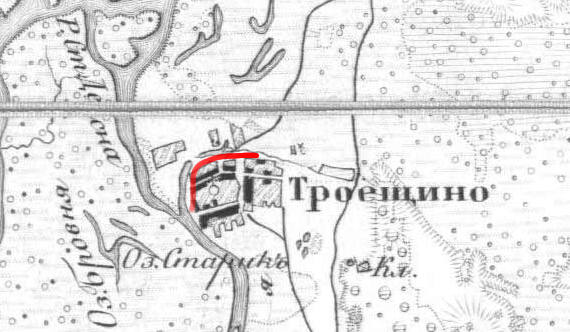
\includegraphics[width=\linewidth]{chast-gorodki/star-ist/radunka-kovbanka.jpg}
\end{center}

Сказано, что Радунка отходила в сторону от  речки, которая начиналась в Днепре. А ведь сейчас между Днепром и местом «старой» Троещины, на острове Муромце лежат явно старицы чего-то, долгие озера Кинище и Малое Кинище. Не они ли остатки русла, описанного как «речка виходячая з днепра»?

Но продолжим разбор. Про Радунку: «тею речкой вменяючи еи за долину провадили менование два человеки чрез село Троеччину аж до озерца которе впадает в чорторию».

%Уже на широте Троещины встречаем упоминание Черторыи, в которую впадает некое озерцо. Значит, тогда Черторыей именовалось некое русло, близкое к Радунке.

Полагая «тою речку» (Радунку) за «долину» из давнего ограничения земель, два старожилы проводили комиссию через село Троещину до озерца, впадавшего в Черторыю. Неясно, севернее ли Троещины это озерцо или южнее, и соединено ли с Радункой.

Однако вывод – тогда Черторыей именовалось некое русло, близкое к Радунке, на широте примерно Троещины.

\begin{quotation}
там пришовши не питано их ведлуг ограниченя дворецкого жебы провадили чрез речку Радунку, леч питано зараз покажете врочище старое кладовище,
\end{quotation}

Там старожилов не просили, согласно ограничению полковника Дворецкого, провести комиссию через речку Радунку, но лишь попросили показать сейчас урочище Старое кладовище.

\begin{quotation}
а тогда тие два человеки повидели их неведают где старое кладовище, леч показали им новое, на край борка троецкого з долины входячи от троеччины в борок при дорозе, 
\end{quotation}

Тогда два старожилы свидетельствовали, что не знают, где Старое кладовище, а лишь показали комиссии новое, у края борка троецкого, выходя из долины от троещины в борок при дороге.

\begin{quotation}
до того кладовища нового поступаючи от озерца понад долину полем зеленым питали викгуровских людей если они орут, албо орали когда тое зеленое поле, отповедали иж не орали на том месце ныкогда, бо из троеччины люде навесне збегают под борок для великой воды, 
\end{quotation}

Комиссия, идя к новому кладбищу от озерца, над долиной зеленым полем, спрашивала у викгуровских людей, пашут ли они, либо пахали когда то зеленое поле? Те отвечали, что не пахали на том месте никогда, ибо из Троещины люди весной спасаются у борка от половодья.

\begin{quotation}
тым полем зеленым понад долиною йдучи помимо новое кладовище припровадыли до трох груш где отец намстник Михайловский одозвался до отца игумна троецкого мовичи, же отец игумен Троецкий ездячи в субботу тижнем перед тим осмотром, показовал, ему тое старое кладовище, якож и не перечил тому слову отец игумен троецкий, где люде обосторонние осмотрили, же при тих трох грушах, и много было груш тилко же позрубание, яко видат еще й пне й лежачие рубание груши, а кладовище от людей троецких поораное й посеяное, що позабрнаю тоей пашне явно и достоверно показовалося.
\end{quotation}

Тем полем зеленым над долиной идя мимо нового кладбища прошли до трех груш (урочище), где наместник Михайловского монастыря обратился к игумну Троецкому, что отец игумен Троецкий, отправившись в субботу за неделю до нынешнего выезда комиссии, показывал ему то Старое кладовище. Игумен Троецкий не возразил.

У трех груш представители обеих сторон увидели, что около тех трех грушах было много других груш, только срубленных – они валялись еще порубленные, да торчали пни. А кладовище (вероятно, урочище Старое кладовище) оказалось троещинскими людьми вспаханным и засеянным.

\begin{quotation}
От того врочища старого кладовища хотичи поступити ку врочищу городищу порожнему подле борка где замочок и двор был князя Семена Олельковича
\end{quotation}

От того урочища Старого кладовища хотели подойти к урочищу Городищу пустому, возле борка где были замочек и двор Олельковича.

\begin{quotation}
питано чий там кгрунт отновидели единогласно так троецкая яко й викгуровская громада иж влево под борком троецким троецкие кгрунта, а вправо здавна як кто зазнал, все викгуровские кгрунта з которых насланние игуменские троецкие забрали жито 
\end{quotation}

Был задан вопрос, чей там грунт? Единогласно отвечали троицкая и викгуровская громады, что влево под борком троицким – троицкие грунты, а справа издавна, как кто вспомнил (зазнал), все грунты выгуровские, с которых посланцы игумена троецкого и забрали жито. 

\begin{quotation}
й так старою дорогою понад борок проважене ведут права обоего к уменованному врочищу городищу порожнему, от того городища олелькова проважено понад борок троецкий на поле прудец 
\end{quotation}

И так старой дорогой через борок, «права обоего» (как указана граница в земельных документах обеих сторон) ведут к упомянутому городищу пустому, а от того Олелькова городища, через борок троецкий на поле Прудец.

\begin{quotation}
тут отец економ михайловский отозвался мовячи понеже в правой руце ведлуг права кгрунти викгуровские тройчане их позасевали, теди слушная речь брати у ных десятину до монастыра михайловского, 
\end{quotation}

Тут эконом Михайловский сказал, что поскольку справа, согласно документам размежевания – грунты викгуровские, а тройчане их засеяли, то правильным будет брать с них десятину на Михайловский монастырь.

\begin{quotation}
тое тройчане почувши чим борзей почали звожовати пашню додому, же на утрейший день мало що зосталося, 
\end{quotation}

Услышав это, тройчане поскорей начали увозить хлеб домой, и наутро мало что осталось.

\begin{quotation}
а от прудца проважено до трох курганов, от трох курганов долиною около стойла йли мимо селище, бо тут питано людей щобо то было за стойло?
\end{quotation}

От прудца провели комиссию до трех курганов, а от них долиной возле стойла или селища, и тут спросили у старожилов, что за стойло такое было? Иными словами, комиссия не понимает, что называть стойлом, что за урочище такое?

\begin{quotation}
отповидали люде, иж там тройчане на весне збегают перед половодьем, и стоят там аж до святого Николая поки води опадает, 
\end{quotation}

Люди отвечали, что тройчане собираются перед половодьем и живут там, «стоят» до дня святого Николая, пока воды не спадут.

Про то, что давнее урочище было «стойлом татарским», никто не вспоминает. Быть может, показали какое-то другое «стойло».

\begin{quotation}
там же доводили того и пустим колодезищем до того стойла проважено на конец кривой нывы долиною живцем аж у речку угнор власне до того мейсца поки спор между обема сторонами, 
\end{quotation}

Там же доказывали это, и мимо пустого колодезища (место высохшего колодца) прошли в конец кривой нивы долиной живцом в речку Угнор собственно к тому месту, за которое спорят обе стороны.

\begin{quotation}
оттоль все совокупне поступили через менованное зеленое поле знову ку троеччине и через село переехавши, 
\end{quotation}

Оттуда все вместе перешли через названное зеленое поле снова к Троещине и проехали через село.

\begin{quotation}
а станувши над оною Ковбанкою где речка Радунка закрывилася в село Троеччину домишлялился з стороны Михайловской же треба было ведлуг ограничення йх п. Дворецким учиненного, перейти через речку Радунку аж на конец поповой сеножати, до озерца що впадает в Чорторию ведлуг которого ограничения уважаючи по слушности й по благой совести признаючи, це ле на кгрунте милославском, то есть викгуровском стоит троеччина ново осаженна, 
\end{quotation}

А остановившись над Ковбанкой где речка Радунка поворачивает в село Троещину, сторона Михайловская заметила, что надо было, согласно ограничению их, произведенному паном Дворецким, перейти через речку Радунку на конец поповой сеножати к озерцу, что впадает в Чорторыю, в силу ограничения признавая, что «новоосаженная» Троеччина (то есть возникшее, новое поселение) стоит на земле Милославской, то есть Викгуровской.

\begin{quotation}
Кгдыж опрочь того ограничения дворецким учиненного, й монастыреви Михайловскому служачого, еще старинный человек йменем Герасим Матвеевич перед Каменеччиною\footnote{Быть может, речь идет о взятии Турками крепости в Каменце-Подольском в 1672 году?} близко пяти десять лет до Викгуровщины зашлый под сумненем поведил,
\end{quotation}

Помимо того ограничения Дворецкого, свидетельствующего в пользу монастыря Михайловского, еще и старожил Герасим Матвеевич, поселившийся в Викгуровщине за 50 лет до Каменеччины, подписью своей удостоверил показание:

\begin{quotation}
иж он две тилько застал хаты, на сем боку того озерца где троеччина едину Чечужину, а другую Лукянову, который Лукян зайшол был Барышполя, и поселился был на сем боку озерца над чорториею, леч уже тое месце знесла Чортория, а на другом боку озерца, где Троецкий кгрунт там тилко три хате было, една Копилева, а другая Семена Павленка, а третая Ивана Молина, что слишачи мененого Лукяна сын признал же так было а не йначей.
\end{quotation}

Что он застал только две хаты на этой стороне того озерца, где Троещина – одну хату Чечуги, а другую Лукьяна, который перебрался сюда из Борисполя и поселился на этой стороне озерца над Чорторыей, однако ныне то место уже снесла Чорторыя. А на другой стороне озерца, где Троицкий грунт, там только три хаты было – Копыла, Семена Павленка, да Ивана Молина. Услышав это, упомянутого Лукьяна сын подтвердил, что было так, а не иначе.

\begin{quotation}
Любож хотели Михайловские через речку Радунку ведлуг ограничения Дворецкого, и ведлуг права Троецкого осмотрити конца поповой сеножати, и озерца над Чорториею там впадаючего, еднак кгды уже было близко ку вечеру, а отец игумен троецкий з своими настоял, жебы того ж дня и ведлуг их людей признати могл ся показати дукт ограниченя.
\end{quotation}

Представители Михайловского монастыря хотели, согласно ограничению Дворецкого отправиться через речку Радунку, и по «праву» Троицкому осмотреть конец поповой сеножати да озерцо над Чорторыей там впадающее. Однако дело было уже близко к вечеру, а игумен Троицкого монастыря настоял, дабы сегодня же продолжили принимать свидетельства их людей, которые могут показать показать линию размежевания (дукт ограниченя).   

\begin{quotation}
Прето отцеве Михайловские на инший час собе тое откладаючи, сойзволили, и поступили отоль все ку реце Гнылуши, которую назвавши Тройчане Радункою, далей пошли понад тоею ж ку порожнему городищу князя Семена Олелковича.
\end{quotation}

Представители Михайловского монастыря отложили задуманное на другое время, и согласились с троицкими. Все пошли оттуда к реке Гнылуше, которую тройчане назвали Радункой. Дальше двинулись над нею к пустому городищу князя Олелковича.

Важное указание, что тройчане отождествляли Гнилушу с Радункой! Вдоль указанного русла можно было выйти к пустом городищу Олелковича. Документ, составленный несколько с точки зрения представителей Михайловского монастыря, кажется сомневается в том, что Гнилуша это Радунка, ведь тогда граница проходит совсем иначе, нежели выгодно «михайловским».

Суть препирательства в этой части протокола – михайловские называют речку около «городища» Гнилушей, тройчане же – Радункой. В ограничении, в частности поля Чуриловского, что принадлежит Троицкому монастырю, граница проходит по Радунке, а не по какой-то Гнилуше. Именуя Гнилушу Радункой, тройчане передвигают границу, захватывая поле (вероятно, на западном берегу нынешней Гнилуши) в свои владения.

Вот почему михайловские упорно просят – покажите нам именно Радунку. Им же показывают другую, с точки зрения михайловских, речку – Гнилушу.

\begin{quotation}
Кгды зась отцеве Михайловские просили отцев з троецкой стороны, жебы провадили через Радунку отповидели не глядете вы на права идете вы тилко за нами куда вас попровадим, и от той Гнылуши которая попод самое порожнее городище олелковичово идет вишли на вал того городища, з которого не хотели Михайловские зийти аж бы отец игумен Троецкий ведлуг права своего показал вперед дукт через тую Радунку, а долиною жебы провадил ку кладовыщу, а от кладовыща аж в той час ку тому городищу олелковичовому а не на самое городище випровожал;
\end{quotation}

Здесь отцы Михайловские просили отцов с Троецкой стороны, чтобы те провели через Радунку, на что Троецкие ответили – не глядите на права (документы с описанием границ), а идите только куда мы вас поведем.

И от той Гнылуши которая под самым пустым городищем Олелковичевым идет, вышли на вал того городища, с которого не хотели Михайловские сойти, пока игумен Троецкий, согласно документу своему не показал бы сперва границу через ту Радунку, а долиной чтобы проводил к кладбищу, а от кладбища тотчас к тому городищу Олелковичому, а не на само городище выводил.

Михайловские, сомневаясь в правильности показаний границы, просят троицких провести комиссию последовательно через все эти урочища, как они записаны в документы. Вероятно они полагают, что если Гнилуша это не Радунка, то подобный маршрут будет невозможен.

\begin{quotation}
При том довольном споре на валу Городища Олелковичовскаго Гришко Прохоренко Родимец, а Демко Сердюков брат зайших под час Каменеччины Троеччянские жители спитанние, чие бы то поле было за тим Городищем Олелковичовым, где забрано жито Викгуровское, и побито городничого Иеромонаха Иакинфа;
\end{quotation}

Во время сего спора на валу Городища Олельковича, Гришко Прохоренко Родимец, и Демко брат Сердюка – жители Троещины, осевшие тут во время Каменеччины, были спрошены, чье это поле было за тем городищем Олельковича, где забрано жито викгуровское и побито городничего иеромонаха Иакинфа?

\begin{quotation}
Отповидали под сумненем доброволне иж як запамятали то всегда там Викгуровщане орували, яко теперь аж под самую Троеччину, якое признате годных веры людей учувши всенародно призвано иеромонаха Иакинфа, и обнаживши до пояса показанова нещадное побитье на правой руце ку плечам барзо тело перебитое кровью закипелое, а з заду до по хребту подобное побятие в килкох месцах, того не слушного дествия отец Игумен стидячеся и жалуючи з воздыханием приказал побранное насланими своими жито зараз отдати, а отцу Иакинфу городничему побитому, за подертую рясу обецал целую дати и боль нагородити по совершенно дасть Бог ограниченю, а тих насланних своих важившихся так нещадно бити городничого, при притомности его в манастиру троецкому четвертого дня значне скарати.
\end{quotation}

Старожилы показали, что жители Викгуровщины всегда там пахали, как и теперь, под самую Троещину.

Затем явился иеромонах Иакинф и обнажил раны. Устыдившись действий своих людей, игумен Троецкий приказал отобранное жито отдать, а иеромонаху за порванную рясу обещал целую.  Испытанную боль игумен вознаградит по окончанию ограничения, учинивших же избиение существенно покарает, когда сам четвертого дня вернется в монастырь.

\begin{quotation}
По тому уговору отец Игумен Троецкий просил жебы далей глядети врочищ, и попровадил через Векгуровщину село по мимо дворец до млынка стоячого подле дворца и повидел отож й прудец.
\end{quotation}

Пообещав это, игумен Троецкий просил чтобы продолжить смотр урочищ, и повел через село Векгуровщину мимо дворца (главный двор села, «помещичий») до млынка (водяной мельницы), стоящей подле дворца, и свидетельствовал – вот же и прудец!

\begin{quotation}
Тут питано з стороны Михайловской отца Игумена Троецкого, если то прудец врочище, чи ли з московска по Великороссийску подобно словне прудец млыном зовется?
\end{quotation}

Тут Михайловская сторона спросила игумена Троецкого – если это урочище Прудец, то разве по-московски на великороссийском языке слово «прудец» переводится как «млын»?

\begin{quotation}
На тое отец Игумен замолчал, а отец економ Печерский на коня всевши поехал передом з людми и зъехавши з дороги на трое албо на четверо гоны невеликие\footnote{Гон, гоня – 120 сажень. Чему равна «гона невеликая», то есть малая, я не знаю.}, безпутя провадил, и запровадил межи такую гущу и коренье в березник и добчак, же немещно было далей поступити,
\end{quotation}

На то игумен промолчал, а эконом Печерский, усевшись на коня, поехал вперед с людьми и, сойдя с дороги на три или четверо гоны небольшие, повел комиссию без разбору и завел ее в такую гущу, березняк и дубраву, что нельзя было двигаться дальше.

\begin{quotation}
А так просили Михайловские отцеве звыежджими жебы албо от врочища до врочища провадил показуючи кгрунта, з едного боку левого троецкие яко ведется и яко в праве вписано, албо жебы отложити наутрейший день, бо уже пришло было слонце на запад.

По согласию теды обоих сторон отложено той осмотр з пятници на утрейший день суботный.
\end{quotation}

По просьбе Михайловских отцов, которые настаивали на последовательном смотре урочищ и сверке их с «правами», по согласию обоих сторон, смотр перенесли с пятницы на утро следующего дня, ибо солнце почти зашло.

\begin{quotation}
В Суботу, числа 29, месяца того ж июля, зъехавшися в дворец Выкгуровский, а з дворца согласившися знову выехали на вчорайшое месце до порожнего городище олелковичового, и там ставши на валу читано обоих сторон права менованние вышше, а зишовши з городища поступили все громадно на сеножат над Чорториею лежачую, межи речкою Радункою, и межи речкою Гнылушою.
\end{quotation}

В субботу 29 июля комиссия и стороны съехались в дворец в Выкгуровщине, оттуда, посовещавшись, снова отправились на вчерашнее место к пустому городищу Олельковича, и став там на валу, было зачитано обеих сторон права. Сойдя с городища, все толпой пошли на сеножать, лежащую над Чорторыей, между речкой Радункой и между речкой Гнылушей.

Если толковать буквально «над», то сеножать – к северу от Черторыи, однако при этом между речками Радункой и Гнилушей. Если не буквально, то сеножать где-то на берегу Черторыи, а с двух других сторон этой сеножати – речки Радунка и Гнилуша.

\begin{quotation}
Там отец економ печерский читал писмо якоесь старинное, в котором описано як небожчик Выкгура вдралася через Угнор в Чуриловщину в поле церковное легкованное старцам болницким троецким.
\end{quotation}

Там печерский эконом читал какую-то старинную бумагу, где описывалось, как покойник Выкгура «вдрался» за Угнор, его пределы, к Чуриловщине – полю, пожалованному во владение (легкованное – от «legatio», запись в актовой книге, передающая право собственности на что-либо) Троицкому Больницкому монастырю.

\begin{quotation}
З тоей окказии отцеве Михайловские просили, абы отец Игумен Троецки изволил показати им тое поле Чуриловское за Угнором, поневаж то о него и перед тим бывал, и теперь есть спор. Отец Игумен показал им на тое поле що за городищем, ото тое поле що Чуриловщина. 
\end{quotation}

По этой причине отцы Михайловские просили, чтобы игумен Троецкий изволил показать им то поле Чуриловское за Угнором, ибо о нем и ранее, и ныне идет спор. Игумен показал им на то поле, что за городищем, что оно и есть Чуриловщина.

\begin{quotation}
Тут обе стороне согласившися усоветовати питати, если кто з троецкой громады албо з векгуровской признает, и назовет тое поле за городищем Чуриловщиною?

И так двох мужей старинных позвавше з громади векгуровской питанно под сумненем як оны тое поле называют?
\end{quotation}

Обе стороны, посовещавшись, решили спросить у кого-нибудь из троецкой или векгуровской громады (населения), известно ли им это поле за городищем как Чуриловщина?

И позвав двух старожилов из громады векгуровской, спросили их, как они то поле называют? 

\begin{quotation}
Отповедили кленучися же а ни сами, а никто иный з посторонных людей називают иначей, тилко когда трафится так мовят до своих домашных, выженте товар за городище старое 
\end{quotation}

Отвечали, клялись, что ни они сами, и никто из посторонних людей особо никак не называет, разве что когда надо говорят своим домашним – выгоните скотину за городище старое.

\begin{quotation}
подобне позвавши двох мужей з троецкой громады, питано о том полю за городищем чи не чули от кого як бы то ся тое поле где побрано жито називало?

Отповидели так же слово в слово иж не чули, абы кто иначей називал, толко поле за городищем.
\end{quotation}

Подобно вызвав и двух человек из троицкой громады, спрашивали их о поле, что за городищем, не слышали ли от кого, как то поле, где забрали жито, называется?

Отвечали слово в слово, что не слышали, чтобы кто называл иначе, чем «поле за городищем»

\begin{quotation}
Аж тут отец економ печерский офукнулся на свою громаду троецкую мовячи, а чи глухии былисте як читано же то Чурилковсщена. Тут отцеве Михаиловские долго просили, и спиралися, жебы им показал отец Игумен тую Чуриловщину, о которой спор.
\end{quotation}

И тут отец эконом Печерский прогневался на свою громаду троецкую, говоря – а вы глухие были, когда я зачитывал бумагу, что то Чурилковсщена? 

Тут отцы Михайловские долго просили и спорили, чтобы отец игумен показал им ту Чуриловщину, о которой спор.

\begin{quotation}
А в тим житель Троецкий Кондрат козак примовил отцу економу Михайловскому тими словы: що ти спираешься неверный жиде.

За якую примовку зараз отец економ печерский того козака лежачого на земли кием три разы ударил и скарал. А козак Кондрат оскобленный з завзятости своея вирекл тие слова отож я тепер попроважу где радунка.
\end{quotation}

При этом житель Троецкий, козак Кондрат сказал эконому Михайловскому – что ты возражаешь, неверный жид.

За эти слова отец эконом Печерский немедленно того козака, на земле лежащего, кием три раза ударил. А козак Кондрат, оскорбленный, в запале изрек – ну я теперь проведу Радункой.

\begin{quotation}
И любо просили отцеве Михайловские, жебы той разъяренный человек не провадил, леч таких два которые бы сумлением обовязании, и добре ведаючи врочища. 
\end{quotation}

И очень просили отцы Михайловские, чтобы тот разъяренный человек не «провадил» – не показывал урочище речку Радунку, но речку показывали два таких свидетеля, что под письменной присягой и хорошо знают урочища.

\begin{quotation}
Однакож отец Игумен Троецкий з отцем економом печерским жадали, абы той человек велце им потребный показывал врочища, и так дошли до речки Гнилуши где повидел той Кондрат жител троецкий иж то Радунка где вода течет а Гришко Троецкий же житель повидел аж то Радунка где долинка видалася, понад тую Гнилушу, 
\end{quotation}

Но игумен Троецкий с отцом экономом печерским желали, чтобы тот человек (козак Кондрат), весьма им нужный, показывал урочища.

И так дошли до речки Гнилуши, где тот житель троецкий Кондрат свидетельствовал, что это Радунка, где вода течет. А Гришко, тоже житель Троещины, свидетельствовал, что Радунка это где долинка получилась, вдоль той Гнилуши («понад» можно перевести и как «выше» – вероятно северней).

\begin{quotation}
а викгуровщяне единогласно твердили иж то за их памяти небожчик Игумен Михайловский Силвестр Головчич тую Гнилушу велел роскопати, хотячи туда Чорторию пустити, чтобы мощно живцом з викгуровщини водным судном провадити до Днепра.
\end{quotation}

А викгуровщане единогласно утверждали, что на их памяти, покойный игумен Михайловского монастыря Силвестр Головчич ту Гнилушу велел раскопать, желая пустить туда Чорторыю, чтобы можно было по «живцу» из Викгуровщины водным судном добраться до Днепра.

Это загадочное свидетельство, которое толкуется по-разному. Возможно, игумен хотел соединить каналом Черторыю с Гнилушей, чтобы из последней добираться по Черторые в Днепр.

Поскольку сейчас, в этом документе, всё крутится возле Троещины и Выгуровщины, предположу, что Черторыей тогда считался позже пересохший и распавшийся (на Кинище и прочее) рукав от Днепра через остров Муромец. 

\begin{quotation}
Видячи тое, отцеве михайловские, же един з завзятости своея провадит, а другий иначей повидает и не згажаются тие вози, просили жебы тое несогласие их записати, там же тое записавши, просили отцеве михайловские, чтоби отц игумен велил провадити ведлуг права своего через Радунку тую, отповидил отц игумен троецкий, не можно провадити, бо там через Радунку их михайловские синожати, и тое записати михайловские хотили, же не ведено через Радунку ведлуг своего права, леч отц игумен з своими боронил того и чим борзий от тоей Гнилуши, которая попод городище Олелковичово течет, вишли зараз наверх городища, не ведучи ведлуг права, яко там описанно через Радунку, а оттол долиною ку кладовищу, а от кладовища подле борка ку городищу.
\end{quotation}

Отцы михайловские, видя, что один дает показания из-за своей «завзятости», а другой иначе, и между собой свидетельства не согласуются, просили, чтобы то несогласие, расхождения были записаны.

Там же записав, отцы михайловские просили, чтобы отец игумен провёл согласно своим правам через ту Радунку, но игумен ответил, что нельзя провести, ибо там через Радунку – михайловские сеножати.

Представители Михайловского монастыря хотели это записать, что игумен не провел их через Радунку согласно «праву». Но игумен воспрепятствовал этому, не дал записать, и как можно скорее от той Гнилуши, которая течет под городищем Олельковича, вывел сразу на верх Городища, не согласуясь с документом, где описано «через Радунку а оттуда долиною ко кладовищу, а от кладовища подле борка к городищу», то бишь не была пройдена вся заданная в документе последовательность урочищ.

\begin{quotation}
А кгды не хотячи з городища далее поступити, отцеве Михайловские, домогалися того жебы конечне отец Игумен Троецкий провидил их ведлуг права своего по врочищах.
\end{quotation}

И там отцы Михайловские, не желая далее двигаться с городища, требовали, чтобы игумен Троецкий наконец провел их согласно «праву» своему по урочищам, показал их.

\begin{quotation}
А он видячи при всем народе, же це ле не может показати, бо не было там жадных таковых признаков, тилко все збивали тим иж тут же й долина тут и кладовище тут же на едном месцу и Городище, шепнувши собе щось до уха, оставили отцев Михайловских звиежджими на Городищу, а сами поступили далей под Борок, отцове Михайловские собе ж восвояси ку дворцу своему пустилися.
\end{quotation}

А он понимая при всём народе, что не может этого показать, ибо не было никаких таких признаков урочищ, только всё путал, сбивал тем, что тут же и долина, тут и кладовище, тут же на одном месте и Городище. Троецкие отцы, пошептавшись, оставили отцов Михайловских на Городище, а сами переместились дальше под Борок. Отцы же Михайловские уехали восвояси к своему «дворцу» в Викгуровщине.

\begin{quotation}
Отец зась Игумен Троецкий з своими отъехавши на гони добрий прыслати на дорогу под селом до отцев Михайловских абы без спреки изволили за ними изыйти куда провадят, й так по их изволению приехавши к ним отцем, отцеве Михайловские отозвалился з тим, чому по вчорашйшому не провадите через село Викгуровщину, не укрывжайте монастыра Михайловского, покажете врочище Прудец подле Борка, отповидели з стороны Троецкой, есть там в селе Прудец, а было от того месца з под Борка до Млынка в селе стоячого далеко ити на добрие двое гоны.
\end{quotation}

Игумен Троецкий, отъехав со своими на добрую гону, послал на дорогу под селом к отцам Михайловским, чтобы изволили за ними ехать куда проведут.

Те согласились и, прибыв к троецким, спросили – почему не проведете, как вчера, через село Викгуровщину? Не обижайте монастырь Михайловский, покажите урочище Прудец подле Борка. На что с троецкой стороны ответили – есть там в селе Прудец, а от того места из-под Борка, до Млынка, стоящего в селе, далеко идти, на добрые две гоны.

\begin{quotation}
От того месца отец економ печерский верхи передом провадил з початку по под борок, а далей удалился вправо, и перейхали через якуюсь речку, и тую речку живцом назвавши, провадили водою а не долиною живцем, як в их праве троецком описанно же долиною живцем а не водою живцем, и так ездили не попод борок около стойла леч обездили нывы пашенние в правой руце оподаль от борка Троецкого так далеко, иж в иншому месцу ледве их оком мощно было зглянути, а то знат для того, жебы з тых ныв, тройчанами посиянных, и з ных пожиткуючи, отц економ михайловский не забирал десятину, з чим вчорайшого дня пятничного перед всими на поли прудци подле борка оповищался.
\end{quotation}

От того места эконом печерский, верхом, сначала провёл комиссию под борок, а затем удалился вправо, и переехав через какую-то речку да назвав ее «живцом», провел водой, а не долиной живцом, как в их праве троецком описано долиною живцом, а не водою живцом. 

И так поехали не под борок около стойла, но лишь объехали нивы пахотные по правую руку в отдалении от борка так далеко, что кое-где едва были заметны. И это снова для того, чтобы с тех нив, тройчанами засеянными, отец эконом Михайловский не забирал десятину, как вчера в пятницу предлагал перед всеми на поле прудце возле борка.

Отмечу, что в протоколе урочище Прудок рассматривается не как водоем, но как некое «поле Прудок», поскольку признание урочища прудка прудком, показанным в Выгуровщине, означало бы, что Выгуровщина ощутимо залезла на троицкую землю.

\begin{quotation}
А так обехавши тие нивы совокупилися над Угнором при концу Кривой Нывы. Где отец економ Печерский ставши отзивался з тим, абы отцеве Михайловские не важилися против зимы пахати того поля за городищем Олелковичовым. А отцеве Михайловские взаемне протестовалился, абы тройчане не важилися тых ныв объеханных пахати. Кгды ж и ведлуг права троецкого и ведлуг Дворецкого ограниченя в правой руци подле борка милославским людем перед тим, а тепер викгуровщаном михайловским, кгрунта
належат.
\end{quotation}

Объехав таким образом те нивы, собрались на Угнором на конце Кривой Нивы. 

Там отец эконом Печерский стал настаивать, чтобы отцы Михайловские перед зимой не смели пахать то поле за городищем Олелковича. 

А отцы Михайловские в свою очередь возражали, чтобы тройчане не смели тех объеханных нив пахать – поскольку и согласно праву троецкому, и ограничению Дворецкого, по правую руку возле борка грунты принадлежали сначала милославским людям, а теперь выкгуровщанам михайловским.

\begin{quotation}
А тие кгрунта, попустивши тройчаном, осилым на кгрунти выкгуровском, ци ле бых Выкгуровщину назвати трудно Викгуровщиною, хиба Троеччиною, бо вси кгрунта около борка в правой руци не ведлуг права свого, леч против права пашут тройчане и, яко мовят, же оны и отци их тими владили нивами и орали оние, тое по правди говорят. 
\end{quotation}

А те грунты, где попустили тройчанам осесть на грунте выгуровском, трудно назвать Выкгуровщиной (землей с таким именем), разве что Троещиной. Ибо все грунты около борка по правую руку, не по «праву», но вопреки, пашут тройчане, истинно утверждая, что они и отцы их владели теми нивами и пахали их.

\begin{quotation}
Кгди ж всивши отци их новоосаженую Троеччину на кгрунти михайловском по сем боку озерца, впадаючого над Чорторию, то негде инде подитися им, тилко тиеж викгуровские кгрунта мусят пахати и тим препитатися. 
\end{quotation}

Потому что когда отцы их поселились на новосозданной Троещине на грунте михайловском по этой стороне озерца, впадающего над Чорторыей, то негде им больше было пахать для пропитания, кроме тех же викгуровских грунтов.

Далее следует заключительная часть протокола комиссии, с подписями и уверениями, что всё записано как было увидено и услышано, не отдавая предпочтения ни одной из сторон. Хотя по документу видно, что одной таки отдано.

\begin{quotation}
На яком осмотри урочищ, вижей описанных, по блгословению преосщенного пастира его милости и всечесного его млсти отца архимандрита Киево-Печерского изволению з послушаниа стого бывши ми притомными, щосмо слишали и видили очима нашима, тое все поистинни списавши, не уводячися жадним респектом сторон, маючих спор межи собою о тие кгрунта для учиненя реляции пославшим нас и для липшой информации тим, мают совершенную на суди децизию, по сем ограниченю часу постановленного чинити з должности ншой при печати консисторской митрополитанской киевской и при подписи рук нших власных подалисмо. 

Писано в катедри митрополитанской сто-Со\-фийс\-кой киевской. При сем розыску и цило утверженной по правам граници подпис рук власных вираженых, иеромнах Товия Петрашко, казнодия, судия консисторийский, судов метрополии киевских дхвных. 

По едной сторони печати, а по другой иеромнах Евстратий, писар дховных судов метрополитанских киевских. Для липшой теды в потомное времена твердости в книги судовие заведши, сей випис з суду войскового енералного з подписом руки, с притисненем печати судовой видано в Глухови року, мсца и дня више вираженного.

Его царского пресвитлого величества Войска Запорожского енералный судиа Алексий Михайлович Турянский
\end{quotation}

В том же году, когда комиссия смотрела земли и велась тяжба, у старожила-рыбака Василя Закгуры выясняли, где же протекают речки Радунка и Гнилуша. В фондах библиотеки имени Вернадского нашелся следующий документ\cite{mihdocs}:

\begin{quotation}
Выпис з книг миских права майдебурского, ратуша киевского. Року тисяча семьсот четвертого, мсця августа второго дня.

Его црского прсвтлого влчства в ратушу киевском перед нами, Димитрием Полоцким, упривилиованным войтом, а Иосифом Корниевичом, рочним бурмистром и перед райцами и лавниками, ставши персоналитер велебные в Бгу отцы, отц иеромонах Иларион Жикалевич и отц Николай иеродиякон, економ, законники мнстря свтого Михайловского Золотоверхого киевского, именем всее того мнстира братии, зостаючие тепер под властию и началством ясне в Бгу преосвщенного его млсти гспдина отца Захарии Корниловича, епспа
Переясловского, вносили прозбу до ураду, абы Васил Закгура рибалка, старинный жител киевский, был под сумленем спитан, взглядом ричок, еднои текучои под селом Троещиною, а другои под селом Викгуровщиною, о котории рички тепер межи пречестною братиею свтия Лаври Киево Печерския и честною братиею Свто-Михайловскою диется спор.

На которую честных отцев прозбу Васил Закгура кгди был до ураду призван и пытан под сомленем, теды под присягою сознавал, же ричка которая течет под селом Троечщиною, з давных лит называется Радунька, а взялася з рички, называемой Восковицы\footnote{Я не встречал это название нигде более, кроме краткого упоминания в переписных книгах Киево-Печерской лавры за 1666 год: «монастырские села и деревни: Печерского Троицкого больничского монастыря местечко Бровары, а в нем крестьянских 46 дворов, да остров Осетшино, да сельцо Осакорки, да деревня Восковица, да деревня Красиловка» – а где эта Восковица была и как относится к речке, не ведаю.}, и прежными часы упадала у Днипр старик, а як пересипало оную песком, есть тому лит з тридцят, а затонец зарус лопухом, а другая ричка, текучая под селом Выкгуровщиною, называется Гнилушою, взялася з старика Днипра, а упадает у озеро Михайловское. 

Которое Василя Закгуры сознане уряд вислухавши, казал ему сумленем потвердити, а для лит пришлых на прозбу честных отцев свто михайловских велил про памет до книг миских киевских записати, що и есть записано. З которых и сей выпис при подписи руки самого его млсти пана войта и под печатю мискою киевскою есть выдан.

Писан у ратушу киевском, року и дня вышей описанного. Менованный войт рукою власною.
Корыкговал з книгами Иван Пыковскый, писар майстратовый киевский, и подписуюся рукою власною.
\end{quotation}

Изложение сути спора я пропускаю. Закгуру спросили о речках, одна из которых течет под селом Троещиною, а вторая под селом Викгуровщиною. Рыбак под присягой показал, что речка, протекающая под селом Троещиной, издавна называется Радунька, а возникла она из речки Восковицы и прежде впадала в старик Днепра. И лет тридцать назад ее пересыпало песком, залив зарос лопухом, и Радунька в старик Днепра впадать перестала. 

Про речку под селом Выкгуровщина рыбак поведал, что именуется она Гнилушей, происходит из старика Днепра, а впадает в озеро Михайловское.

Старожил-рыбак ни слова не говорит о Черторые! Однако он говорит про «старик Днепр», что может быть проливом от Днепра через остров Муромец, и далее шедшим на юг и вбивающем в себя воды левобережных рек – Радунки и затем Гнилуши.

Этот же «старик Днепр», вероятно, и есть в тогдашнем представлении Черторыя – вернее, верховье оной, северо-западная ее часть. Эта Черторыя устьем никак еще не связана с Десной, Десна пробьется к ней с севера позже. Однако существовал таки рукав Десны (между современной Десенкой и Погребами), что спускался к «старой» Троещине, он-то возможно и был верховьем Радунки. 

Показания рыбака были важны для решения земельного спора, ибо с речкой под Троещиной увязали название Радунки, а к речке у Выгуровщине привязали имя Гнилуши, выведя на бумаге таким образом из частей одной речки – давней Радунки – две разные речки, одну под Троещиной, другую под Выгуровщиной.

Вспомним, как «тройчане» нарицали Гнилушу Радункой. Это их показание не было выгодно Михайловскому монастырю. А вот закрепление имени Радунки за неким бывшим заливом около Троещины отодвинуло границу земель  Троицкого монастыря на север, ибо граница шла по Радунке.

%«Землемер Сноевский», каким-то образом знакомый с этим редчайшим источником –  показанием старожила Василя Закгуры – не пускаясь в проверку на логику всей рисуемой рыбаком картины, делает на основании части этой картины вывод, что «речька же Черторей в древния времена называлась Восковицей». По противоречивой географии Закгуры может и так.

В том же конце 17-го, начале 18 веков, хозяйственная деятельность Михайловского монастыря в Выгуровщине не утихала. Монастырь приобрел дворы Выгуровщины с нивами в смежных урочищах – Сирныковщине и Оболонье, а также «млын лодейный при березе» в самом селе.

Водяные мельницы, млины, в документах того времени делятся на «вальные», «на сваях» и «лодейные». Вальные состояли из нескольких колес, например трех, причем каждое могло иметь отдельного владельца. Лодейные упоминаются «при шлюзе», «при береге», «на рве». Лодейная мельница не требовала для своей работы плотины, ставилась на две лодьи, лодки, выведенные на сильное течение либо на большой реке.

Наличие лодейного млына на Прудке означало, что в этом водоеме было течение достаточно сильное и для устройства мельницы не требовалась плотина. На плане Шуберта, на берегу по другую сторону от церкви через Прудок, тоже показана мельница.

Более документами о Выгуровщине, где не повторялось бы сказанное выше, я не располагаю.
